%[154. - Yue Yi, Zhiqiang Liu, Rong Guo, Ruichen Sun. Design and Implementation of Digital Power Quality Analyzer. – 2016.]

\chapter{Система анализа данных} \label{ch:ch2}

\section{Многопоточность} \label{sec:ch2/sec1}
% Разобраться в том, что такое многопоточность

Система анализа данных(Data analysis System) принимает точные данные из системы сбора и анализа данных. Эта подсистема в основном состоит из частот, гармоник, алгоритма анализа мощности и многопоточности (multi-threading) для повышения эффективности функционирования системы. 

Многопоточность была использована из-за следующих причин:
\begin{enumerate}
	\item Во-первых,АЦП DPQA должны взаимодействовать с пользователями, а это значит, что GUI (Графический Интерфейс Пользователя) должен реагировать за любые внутренние и внешние события. Если применяется последовательное программирование, пользователь может взаимодействовать только с АЦП DPQA, после того как программа завершилась. 
	
	\item Во-вторых, с АЦП DPQA требуется непрерывно получать данные, как только была нажата кнопка «Старт». Многопоточность представляет собой оптимальный способ, чтобы обеспечить обработку данных и одновременного их получения. В заключение, больше времени эффективно применять многопоточность для анализа алгоритмов с участием нескольких операций (т.~е. оконные функции – windowing, промежуточные – padding, FFT и кросс-корреляцию – cross-correlation). 
\end{enumerate}

\section{Алгоритмы расчета частоты} \label{sec:ch2/sec2}

Чтобы рассчитать информацию о качестве электроэнергии, вычисляем сначала входную частоту. Существуют три альтернативных метода для вычисления частоты по дискретизированному сигналу(sampled signal):
\begin{itemize}
	\item Пересечение (Zero-Crossing).
	\item Максимальная точка (Maximum-Point).
	\item Дискретное преобразование Фурье (ДПФ).
\end{itemize}
Метод ДПФ (FFT) используется для вычисления входных значений частоты. Формула ДПФ описана [152]:
% [152 - Sundararajan D. The discrete Fourier transform: theory, algorithms and applications. – World Scientific, 2001.]
\begin{equation}
\label{eq:equation1}
X(k) = \frac{1}{N} \sum\limits_{n=0}^{N-1} x(n)e^{-j\frac{2 \pi}{N}nk}
\end{equation}

где $N$ -- это число $k = 0, 1, \cdots, N-1$

Для реализации ДПФ в Python используем алгоритм быстрого преобразования Фурье (БПФ, FFT). БПФ -- это эффективный алгоритм для вычисления ДПФ (DFT). Число операций необходимых для вычисления Дискретного преобразования Фурье пропорционально $N2$ и $N$ наблюдений при этом алгоритм БПФ требует число операций пропорциональное $Nlog(N)$ [153].
% [153 -	Cooley J. W., Lewis P. A. W., Welch P. D. The fast Fourier transform and its applications //IEEE Transactions on Education. – 1969. – Т. 12. – №. 1. – С. 27-34.]
После того, как реализовали алгоритм вычисления частоты, произошли проблемы разрешением частоты. Для обнаружения потоков сигналов в частотной области,  требуются улучшения разрешения. Сигнал частотной области, рассчитанный БПФ, имеет разрешение $0,5$~Гц. В результате, любое содержимое сигнала, которое существует между двух частот  с разделением $0,5$~Гц, будет полностью игнорироваться, и будет вызван неправильный результат частоты.

Следовательно, разрешение по частоте должно быть улучшено, чтобы минимизировать ошибку вычисления. Используем ноль заполнение для улучшения разрешения БПФ. Из уравнения видно, что длина $X(k)$ полностью зависит от количества образцов $X (n)$.

Текущий сигнал задается уравнением:
\begin{equation}
\label{eq:equation2}
I = R_{HallEffect} \times  I_{ADC} + Offset
\end{equation}

где $R_{HallEffect}$ -- коэффициент выхода напряжения на эффекте Холла;

$I_{ADC}$ -- необработанные текущие данные из АЦП, добавлено смещение, постоянное смещение от схемы регулировки;

Модификация сигнала напряжения:
\begin{equation}
\label{eq:equation3}
V = R_Trans former\times V_ADC + Offset
\end{equation}
где $R_Trans former$ -- Коэффициент обмотки трансформатора;
$V_{ADC}$ -- представляет собой исходные данные напряжения от АЦП;

Из уравнения \labelcref{eq:equation2} длина волны $X(k)$ зависит от количества образцов $X(n)$. Если добавлять нули в конец $X(n)$, способны эффективно увеличить количество образцов $X(n)$ без изменения фактического сигнала. Это будет также увеличивать размер $X(k)$. $X(k)$ не меняется, потому что $X(n)$ остается прежним сигналом. Приращение частоты bins из $X(k)$ мы будем сжимать bins ближе к друг другу, который дает разрешение по частоте.

\section{Алгоритмы вычисления амплитуды гармоник} \label{sec:ch2/sec3}

Содержание гармоник до $20$ гармоники. Содержание гармоник можно извлечь из частотного спектра, после того как мы получили основную частоту БПФ (FFT) напряжения и текущего значения. Гармоники расположены в частотной области, которые являются положительными целыми числами, кратными основной частоте. Чтобы получить гармоники используем частотный индекс и умножаем его на целые числа. После этого берем амплитуды тока и напряжения от БПФ (FFT) на основе рассчитанного индекса. Результаты гармоник не точные (из результатов тестирования). Причина заключается в том, что измеренный нами сигнал ограничен по времени. При выполнении БПФ (FFT), есть частота сглаживания (frequency aliasing). Если заполнять нулями массив, то длина данных увеличивается, и гармоника может не располагать точным частотным индексом (из-за ошибок в вычислениях).

Чтобы решить проблему, вместо использования рассчитанного индекса для получения амплитуды гармоник, ищем индексы. Находим максимальную точку в этом индексе. Тогда максимальная амплитуда будет точкой максимальной амплитуды в пределах диапазона.

\section{Коэффициент мощности и алгоритм расчета энергопотребления} \label{sec:ch2/sec4}

Для нахождения коэффициента мощности была применена перекрестная корреляция (Cross Correlation), а также идентификация триггера (Trig Identity). Перекрестная корреляция нужна для того, чтобы найти более точные результаты идентификации триггера вместо взаимной корреляции. Рассмотрим два сигнала, первый сигнал представляет напряжение из уравнения \labelcref{eq:equation4}, другой~–-~ток из уравнения 

\labelcref{eq:equation5}:
\begin{equation}
\label{eq:equation4}
V = A \cos(\omega t)
\end{equation}

\begin{equation}
\label{eq:equation5}
I = B \cos (\omega t + \theta)
\end{equation}

Ток содержит разность фаз $\theta$. Умножение двух сигналов вместе дает \labelcref{eq:equation6}:

\begin{equation}
\label{eq:equation6}
\left| {V \times I}\right| = \left|A \right| \times \left|B \right| \times \cos \theta  
\end{equation}

Разность фаз может быть найдена как \labelcref{eq:equation7}:

\begin{equation}
\label{eq:equation7}
\theta = \cos^{-1} \frac{V \times I}{A \times B}  
\end{equation}

Уравнение \labelcref{eq:equation7} можно записать в дискретной форме:

\begin{equation}
\label{eq:equation8}
\theta = \cos^{-1} \frac{\sum V\left[ n \right] I\left[ n \right]}{\sqrt{\sum{{\left| V\left[ n \right]\right|}^2} \sum{{\left| I\left[ n \right]\right|}^2}}}
\end{equation}

Функция обратного косинуса может возвращать величину $\theta$, которая означает полярность коэффициента мощности. Чтобы найти полярность коэффициента мощности, используется кросс-корреляцию:

\begin{equation}
\label{eq:equation9}
R_{VI}(l) = \sum_{n=-\infty}^{\infty}V(n)I(n-l)
\end{equation}
где $l=0,\mp1,\mp2,\dots$

$R_{VI}(l)$ -- является наибольшим $l$, в котором напряжение и ток сигнала имеют наибольшее сходство.

Знак перед $l$ показывает является ли коэффициент мощности нагрузки опережающим или запаздывающим. Отрицательное $l$ означает, что текущий сигнал смещен влево. Интервал выборки характеризует отстающую нагрузку. Положительное значение $l$ означает, что нагрузка является ведущей нагрузкой, $l=0$ говорит о том, что нагрузка резитивная (purely resistive). Получение коэффициента мощности позволит рассчитать потребляемую мощность нагрузки.

Из алгоритма нахождения гармоник и амплитуд находим амплитуду содержания гармоник и рассчитываем реальную реактивную мощность в уравнениях (\labelcref{eq:equation10} и \labelcref{eq:equation11}):

\begin{equation}
\label{eq:equation10}
P_{real} = I\times V \cos \theta
\end{equation}

\begin{equation}
\label{eq:equation11}
P_{reactive} = I\times V \sin \theta
\end{equation}

\section{Интерполированные алгоритмы ДПФ с нулевым заполнением для классических окон} \label{sec:ch2/sec5}
% [155. - Luo J., Xie Z., Xie M. Interpolated DFT algorithms with zero padding for classic windows //Mechanical Systems and Signal Processing. – 2016. – Т. 70. – С. 1011-1025.]

Точная оценка параметров (частоты, амплитуды и фазы) для синусоид, загрязненных случайным шумом (random noise), была предметом исследований в различных областях в течение нескольких десятилетий. Например, общая проблема, возникающая при анализе вибрации для вращающихся машин является оценкой параметров дискретизированных многочастотных сигналов в присутствии аддитивного шума (additive noise) [156].

% [156. - Santamaria I., Pantaleon C., Ibanez J. A comparative study of high-accuracy frequency estimation methods //Mechanical Systems and Signal Processing. – 2000. – Т. 14. – №. 5. – С. 819-834.]

С увеличением применения в нелинейных устройствах (non-linear devices) и периодических временных переменных нагрузок в электроэнергетических системах, искажение тока и напряжения сигналов (voltage waveforms) становится серьезной проблемой. Поэтому анализ и контроль гармоник электрической мощности в реальном времени имеет большое значение для поддержания качества электрической энергии (electrical energy), предотвращения повреждения систем электрических сетей (network systems) и экономии энергии (saving energy)[157][158].

% [157.- Zhang F., Geng Z., Yuan W. The algorithm of interpolating windowed FFT for harmonic analysis of electric power system //IEEE transactions on power delivery. – 2001. – Т. 16. – №. 2. – С. 160-164.]

%[158.- Qian H., Zhao R., Chen T. Interharmonics analysis based on interpolating windowed FFT algorithm //IEEE Transactions on Power Delivery. – 2007. – Т. 22. – №. 2. – С. 1064-1069.]
Кроме того, ряд аудио кодирования (audio coding) технологий были недавно разработан, где звуковой сигнал (audio signal) раскладывается на синусоиды и шума перед кодированием. Разложение (decomposition), конечно, зависит от точной оценки частоты (frequency estimation) звукового сигнала [159]. 
% [159.- Ferreira A., Sinha D. Accurate and robust frequency estimation in the ODFT domain //IEEE Workshop on Applications of Signal Processing to Audio and Acoustics, 2005. – IEEE, 2005. – С. 203-206.]

В предшествующей литературе были представлены различные подходы к оценке, которые обычно можно классифицировать на временную область и частотную область. Учитывая их простую работу и высокую эффективность, часто используются подходы в частотной области, основанные на дискретном преобразовании Фурье (discrete Fourier transform – DFT) и реализованные с помощью быстрого преобразования Фурье (fast Fourier transform – FFT). Тем не менее, существуют некоторые присущие методам частотной области недостатки, такие как эффект пикет-ограды (picket fence effect – PFE) и эффект спектральной утечки (spectral leakage effect – SLE) [158]. 
% [158. - Qian H., Zhao R., Chen T. Interharmonics analysis based on interpolating windowed FFT algorithm //IEEE Transactions on Power Delivery. – 2007. – Т. 22. – №. 2. – С. 1064-1069.]

Они могут вносить существенные ошибки в оценки частоты, если сигнал некогерентно дискретизирован (noncoherently sampled) [160][161].

Исследования показали, что если можно позволить себе дополнительные вычислительные затраты, можно компенсировать ошибки и получить высокоточные оценки частоты даже с небольшим количеством выборок [156].
% [156.- Santamaria I., Pantaleon C., Ibanez J. A comparative study of high-accuracy frequency estimation methods //Mechanical Systems and Signal Processing. – 2000. – Т. 14. – №. 5. – С. 819-834.]

Интерполированный алгоритм DFT (IpDFT) является одним из наиболее широко изученных методов оценки [156] ,[157], [158], [159], [160], [161],.[162], [163], [164], [165], [166], [167], [168], [169], [170], [171]. 
% [156.-Santamaria I., Pantaleon C., Ibanez J. A comparative study of high-accuracy frequency estimation methods //Mechanical Systems and Signal Processing. – 2000. – Т. 14. – №. 5. – С. 819-834.]

% [157.-Zhang F., Geng Z., Yuan W. The algorithm of interpolating windowed FFT for harmonic analysis of electric power system //IEEE transactions on power delivery. – 2001. – Т. 16. – №. 2. – С. 160-164.]

%[158.-Qian H., Zhao R., Chen T. Interharmonics analysis based on interpolating windowed FFT algorithm //IEEE Transactions on Power Delivery. – 2007. – Т. 22. – №. 2. – С. 1064-1069.]

%[159.	Ferreira A., Sinha D. Accurate and robust frequency estimation in the ODFT domain //IEEE Workshop on Applications of Signal Processing to Audio and Acoustics, 2005. – IEEE, 2005. – С. 203-206.]

%[160.-Xie M., Adams D. F. A nonlinear finite element analysis for composite materials //Finite elements in analysis and design. – 1996. – Т. 22. – №. 3. – С. 211-223.]

%[161.-Luo J., Xie M. Phase difference methods based on asymmetric windows //Mechanical Systems and Signal Processing. – 2015. – Т. 54. – С. 52-67.]

%[162.-Jain V. K., Collins W. L., Davis D. C. High-accuracy analog measurements via interpolated FFT //IEEE Transactions on Instrumentation and Measurement. – 1979. – Т. 28. – №. 2. – С. 113-122.]

% [163.-Grandke T. Interpolation algorithms for discrete Fourier transforms of weighted signals //IEEE transactions on instrumentation and measurement. – 1983. – Т. 32. – №. 2. – С. 350-355.]

%[164.-Andria G., Savino M., Trotta A. Windows and interpolation algorithms to improve electrical measurement accuracy //IEEE Transactions on Instrumentation and Measurement. – 1989. – Т. 38. – №. 4. – С. 856-863.]

%[165.-Offelli C., Petri D. Interpolation techniques for real-time multifrequency waveform analysis //6th IEEE Conference Record., Instrumentation and Measurement Technology Conference. – IEEE, 1989. – С. 325-331.]

%[166.-Agrez D. Weighted multipoint interpolated DFT to improve amplitude estimation of multifrequency signal //IEEE Transactions on Instrumentation and Measurement. – 2002. – Т. 51. – №. 2. – С. 287-292.]

%[167.-Jacobsen E., Kootsookos P. Fast, accurate frequency estimators [DSP Tips & Tricks] //IEEE Signal Processing Magazine. – 2007. – Т. 24. – №. 3. – С. 123-125.]

%[168.	Belega D., Dallet D. Multifrequency signal analysis by interpolated DFT method with maximum sidelobe decay windows //Measurement. – 2009. – Т. 42. – №. 3. – С. 420-426.]

%[169.-Belega D., Dallet D., Petri D. Accuracy of sine wave frequency estimation by multipoint interpolated DFT approach //IEEE Transactions on Instrumentation and Measurement. – 2010. – Т. 59. – №. 11. – С. 2808-2815.]

%[170.-Duda K. DFT interpolation algorithm for Kaiser–Bessel and Dolph–Chebyshev windows //IEEE Transactions on Instrumentation and Measurement. – 2011. – Т. 60. – №. 3. – С. 784-790.]

%[171.-Schoukens J., Pintelon R., Van Kamme H. The interpolated fast Fourier transform: A comparative study //[1991] Conference Record. IEEE Instrumentation and Measurement Technology Conference. – IEEE, 1991. – С. 358-364.]

Основная идея этого метода заключается в том, что частотная ошибка (frequency error) может быть компенсирована отношением средневзвешенного значения (weighted average) определенного числа известных спектральных бинов вокруг локального максимума. Когда максимум боковых лепестков (sidelobe) выбрано окно распада (MSDW, также известное как Райф-Винсент (Rife–Vincent) класс I окна), ошибка частоты может получить с помощью простых аналитических зависимосытей [166], [167], [168], [169]. 
%[166.-Agrez D. Weighted multipoint interpolated DFT to improve amplitude estimation of multifrequency signal //IEEE Transactions on Instrumentation and Measurement. – 2002. – Т. 51. – №. 2. – С. 287-292.]

%[167.-Jacobsen E., Kootsookos P. Fast, accurate frequency estimators [DSP Tips & Tricks] //IEEE Signal Processing Magazine. – 2007. – Т. 24. – №. 3. – С. 123-125.]

%[168.	Belega D., Dallet D. Multifrequency signal analysis by interpolated DFT method with maximum sidelobe decay windows //Measurement. – 2009. – Т. 42. – №. 3. – С. 420-426.]

%[169.-Belega D., Dallet D., Petri D. Accuracy of sine wave frequency estimation by multipoint interpolated DFT approach //IEEE Transactions on Instrumentation and Measurement. – 2010. – Т. 59. – №. 11. – С. 2808-2815.]

Основываясь на работе Оффелли (Offelli) и Петри (Petri) [165], 
%[165.-Offelli C., Petri D. Interpolation techniques for real-time multifrequency waveform analysis //6th IEEE Conference Record., Instrumentation and Measurement Technology Conference. – IEEE, 1989. – С. 325-331.]
Дуда (Duda) вывел алгоритм интерполяции полиномиального приближения (polynomial approximation interpolation – PAIpDFT), который можно использовать для окон Дольфа-Чебышева (Dolph–Chebyshev) и окон Кайзера-Бесселя (Kaiser–Bessel) [170]. 
%[170.-Duda K. DFT interpolation algorithm for Kaiser–Bessel and Dolph–Chebyshev windows //IEEE Transactions on Instrumentation and Measurement. – 2011. – Т. 60. – №. 3. – С. 784-790.]

Полиномиальные коэффициенты должны быть рассчитаны до анализа, что означает, что коэффициенты для различных окон должны быть рассчитаны и сохранены заранее. Этот процесс неизбежно является интенсивным и хлопотным, особенно для регулируемых окон, свойства которых могут регулироваться одним или несколькими параметрами.

Cначала рассмотрен новый алгоритм интерполяции для окна Хеннинга (Hanning window), в котором был принят метод заполнения нулями, чтобы получить больше спектральных линий (spectral lines) в пределах частотного интервала (frequency interval). Впоследствии этот новый алгоритм был расширен для совместимости с другими классическими окнами путем введения метода подгонки основного лепестка (main-lobe). Изучены систематические ошибки (systematic errors) предлагаемого метода для различных окон, а также характеристики при белом гауссовском шуме (white Gaussian noise).

\subsection{Основы алгоритма} \label{sec:ch2/sec5_1}

Рассмотрим для простоты, но без потери общности, непрерывный косинус-сигнал, загрязненный аддитивным белым шумом, который представлен в виде:
\begin{equation}
\label{eq:equation12}
x(t) = A_0 \cos(2 \pi f_0 t + \theta_0 + e(t))
\end{equation}

где $A_0$ – амплитуда;

$f_0$ – обозначает частоту;

$\theta_0$ – обозначает фазовый угол;

$t$ – обозначает переменную непрерывного времени;

$e(t)$ – белый шум. 

Отбор проб на частоте $f_s$ в течение интервала наблюдения (observation interval) $N\bigtriangleup t(\bigtriangleup t=1/f_s )$, следующий дискретный косинус сигнал $N$ образцы:
\begin{equation}
\label{eq:equation13}
x(n) = A_0 \cos(2 \pi \frac{f_0}{f_s} n + \theta_0) + e(n), n = 0,1, \cdots , N-1
\end{equation}

Чтобы удовлетворить теорему выборки Найквиста (Sampling Theorem), $f_s$ должно быть больше $2f_0$. Разрешение по частоте (Frequency resolution) получается $\bigtriangleup f=f_s/N$ определяется как:
\begin{equation}
\label{eq:equation14}
\frac{f_0}{f_s}=\frac{\lambda_0}{N}
\end{equation}

$\lambda_0$ – обозначает количество циклов, содержащихся в выборках сигнала (signal samples) [169].
%[169.-Belega D., Dallet D., Petri D. Accuracy of sine wave frequency estimation by multipoint interpolated DFT approach //IEEE Transactions on Instrumentation and Measurement. – 2010. – Т. 59. – №. 11. – С. 2808-2815.]

Следует подчеркнуть, что $\lambda_0$ также представляет нормированную частоту (частоту $f_0$, масштабированную по разрешающей способности по частоте), выраженную в бинах DFT [169].
%[169.-Belega D., Dallet D., Petri D. Accuracy of sine wave frequency estimation by multipoint interpolated DFT approach //IEEE Transactions on Instrumentation and Measurement. – 2010. – Т. 59. – №. 11. – С. 2808-2815.]
На этом этапе мы игнорируем шумовой член и переходим к умножению выборок сигнала $x(n)$ на значения окна данных $\omega(n)$.
Взвешенные образцы даны:
\begin{equation}
\label{eq:equation15}
x_\omega(n)=A_0 \cos(\frac{2 \pi \lambda_0 n}{N}+\theta_0)\omega(n)
\end{equation}

Дискретное преобразование Фурье (ДПФ, discrete Fourier transform – DFT) взвешенного сигнала может быть вычислена путем:
\begin{equation}
\label{eq:equation16}
X_\omega(k) = \sum_{n=0}^{N-1} x_\omega(n) e^{-j \frac{2 \pi}{N}nk}
\end{equation}

Применение \labelcref{eq:equation16} к взвешенным выборкам в \labelcref{eq:equation15} дает явный вид~(explicit form):

\begin{equation}
\label{eq:equation17}
X_\omega(k) = \frac{A_0}{2} e^{j\phi_0}W_N(k-\lambda_0)+\frac{A_0}{2}e^{j\phi_0}W_N(k+\lambda_0)
\end{equation}

где $W_N (k)$ и обозначает дискретное временное преобразование Фурье (discrete time Fourier transform – DTFT) весовой функции (weighting function). Если сигнал дискретизируется асинхронно, нормализованная частота $\lambda_0$ находится между двумя самыми большими спектральными линиями (spectral lines). Следовательно, $\lambda_0$  может быть далее записано на две части с целой частью $l_\omega$ и дробной частью (fractional part) $\delta_\omega$ $(-0,5<\delta_{\omega}\leq0,5)$ соответственно.

\begin{equation}
\label{eq:equation18}
\lambda_0 = l_\omega + \delta_\omega
\end{equation}

Целочисленная часть $l_\omega$ может быть легко и правильно определена с помощью процедуры максимального поиска, если SNR превышает пороговое значение (приблизительно от -$18$ до –$20$ дБ) [172]. 
% [172.-Rife D., Boorstyn R. Single tone parameter estimation from discrete-time observations //IEEE Transactions on information theory. – 1974. – Т. 20. – №. 5. – С. 591-598.]
Подстановка \labelcref{eq:equation18} в \labelcref{eq:equation17} дает наибольшую величину:
\begin{equation}
\label{eq:equation19}
\left|{X_\omega(l_\omega)} \right| = \frac{A_0}{2} \left| e^{j\phi_0}W_N(- \delta_\omega) +e^{j\phi_0}W_N(2l_\omega+\delta_\omega) \right| 
\end{equation}

Соответственно, вторая и третья по величине спектральные линии также могут быть определены. При правильной комбинации двух или более спектральных линий может быть получено отношение $\alpha$, которое зависит только от выбранного окна и отклонения частоты $\delta_{\omega}$. Другими словами, если окно данных, как известно, $\delta_{\omega}$ может быть определена только с помощью $\alpha$.

\begin{equation}
\label{eq:equation20}
\delta_\omega = g(\alpha)
\end{equation}

В частности, для максимальных окон распада боковых лепестков (side-lobe) $\delta_{\omega}$ можно записать как функцию от $\alpha$ в простой и явной форме [157], [158], [160], [161], [168], [169].

% [157. - Zhang F., Geng Z., Yuan W. The algorithm of interpolating windowed FFT for harmonic analysis of electric power system //IEEE transactions on power delivery. – 2001. – Т. 16. – №. 2. – С. 160-164.]

% [158.- Qian H., Zhao R., Chen T. Interharmonics analysis based on interpolating windowed FFT algorithm //IEEE Transactions on Power Delivery. – 2007. – Т. 22. – №. 2. – С. 1064-1069.]

% [160. - Xie M., Adams D. F. A nonlinear finite element analysis for composite materials //Finite elements in analysis and design. – 1996. – Т. 22. – №. 3. – С. 211-223.]

% [161.- Luo J., Xie M. Phase difference methods based on asymmetric windows //Mechanical Systems and Signal Processing. – 2015. – Т. 54. – С. 52-67]

% [168.-Belega D., Dallet D. Multifrequency signal analysis by interpolated DFT method with maximum sidelobe decay windows //Measurement. – 2009. – Т. 42. – №. 3. – С. 420-426.]

% [169.-Belega D., Dallet D., Petri D. Accuracy of sine wave frequency estimation by multipoint interpolated DFT approach //IEEE Transactions on Instrumentation and Measurement. – 2010. – Т. 59. – №. 11. – С. 2808-2815.]

Для других окон предлагается решение полиномиальной аппроксимации (polynomial approximation) [170]. 
%[170.	Duda K. DFT interpolation algorithm for Kaiser–Bessel and Dolph–Chebyshev windows //IEEE Transactions on Instrumentation and Measurement. – 2011. – Т. 60. – №. 3. – С. 784-790.]

В следующем разделе представляем простой алгоритм интерполяции (interpolation), который можно применять практически ко всем классическим окнам.

\subsection{Предлагаемый алгоритм} \label{sec:ch2/sec5_2}

Рассмотрим алгоритм техника заполнения нулями. Заполнение нулями – это метод, определяемый как добавление нулевых значений к взвешенным выборкам до вычисления DFT. Добавленные нулевые значения обрабатываются как дополнительные образцы, собранные с той же скоростью, и, следовательно, увеличивают время измерения, как показано в \labelcref{eq:equation21}

\begin{equation}
\label{eq:equation21}
x_{ap}(n)=
\begin{cases}
x_{\omega}, \leq n < N
\\ 0, N \leq n < MN
\end{cases}
\end{equation}

где $(M-1) \cdot N$ добавляются нули. Соответственно, дискретный спектр (discrete spectrum) также расширяется. Эта процедура приводит к более точной выборке спектра сигнала (signal spectrum), потому что вместо $N$ спектральных выборок $M \cdot N$ образцы того же спектра доступны. Обратите внимание, что расширение данных нулями и вычисление более длинного ДПФ действительно увеличивает количество точек в частотной области, но не нарушает основное ограничение и не влияет на эффекты наложения [173].
% [173.-Dorf R. C. Circuits, signals, and speech and image processing. – CRC Press, 2018.]

Пределы разрешения  (Resolution limits) определяются интервалом наблюдения (observation interval) и частотой дискретизации (sampling frequency) [173].

Никакое количество заполнения нулями не может преодолеть эти фундаментальные пределы, и параметры спектра, такие как уровень отношение сигнал/шум (signal-to-noise ratio) и уровень спектральной утечки (spectral leakage), остаются неизменными. Коэффициенты ДПФ по \labelcref{eq:equation21}:

\begin{equation}
\label{eq:equation22}
X(N)= \sum_{n=0}^{MN-1} x_{ap}(n) e^{-j \frac{2 \pi}{N}\cdot \frac{k}{M} \cdot n}, 0\leq k \leq MK-1
\end{equation}
По сравнению с \labelcref{eq:equation16} получается:

\begin{equation}
\label{eq:equation23}
X(k)= X_\omega \left( {\frac{k}{M}}\right)  \end{equation}
Соответственно, \labelcref{eq:equation19} можно переформулировать как:

\begin{equation}
\label{eq:equation24}
\left| {X(l)} \right|   = \frac{A_0}{2}\left| {e^{j\phi_0}W_N(-\delta)+e^{-j\phi_0}W_N \left(\frac{2l}{M}+\delta \right)} \right|,
\end{equation}

где $l$ и $\hat{\delta}
\left( {\delta= \frac{\hat{\delta}}{M}}\right) $
являются целой частью и дробная часть (fractional part) из $M\lambda_0$ соответственно. Точно так же $l$ возвращается максимальной процедурой поиска X(k). На этом этапе три крупнейших линии X(k) даны $\left| {X(l)} \right|$,$\left| {X(l+1)} \right|$ а также $\left|{X(l-1)}\right|$.

Рассмотрим алгоритм интерполяции для окна Хеннинга с техникой заполнения нулями.

Второе слагаемое в правой части \labelcref{eq:equation24} представляет вклад мнимой части (imaginary part) спектра. Если $\lambda_0$ удовлетворяет $5<\lambda_0$ , а также $\lambda_0 < \frac{N}{2}-5$, тогда помехи от второго слагаемого могут быть минимальными и ими можно пренебречь. С этим предположением \labelcref{eq:equation24} сводится к:

\begin{equation}
\label{eq:equation25}
\left| {X(l)} \right| \cong \frac{A_0}{2}\left| {W_N(-\delta)} \right|,
\end{equation}

Точно так же у нас есть это $\left| {X(l)} \right| \cong \frac{A_0}{2}\left| {W_N(\varepsilon -\delta)} \right|$, а так же $\left| {X(l-1)} \right| \cong \frac{A_0}{2} \left| {W_N(\varepsilon +\delta)} \right|$, где $\varepsilon=\frac{1}{M}$. Для окна Хеннинга (Hanning window), $W_N (k) \cong \frac{sin(\pi k)}{h(k)}$,
$h(k) = 2 \pi k (1-k^2)$ [160]
%[160.	Xie M., Adams D. F. A nonlinear finite element analysis for composite materials //Finite elements in analysis and design. – 1996. – Т. 22. – №. 3. – С. 211-223.]

\begin{equation}
\label{eq:equation26}
\left| {X(l)} \right| \cong \frac{A_0}{2} \frac{\sin{(\pi \delta)} }{h(\delta)} ,
\end{equation}

\begin{equation}
\label{eq:equation27}
\left| {X(l+1)} \right| \cong \frac{A_0}{2} \frac{\sin{(\pi \varepsilon - \pi \delta)} }{h(\varepsilon - \delta)} ,
\end{equation}

\begin{equation}
\label{eq:equation28}
\left| {X(l+1)} \right| \cong \frac{A_0}{2} \frac{\sin{(\pi \varepsilon + \pi \delta)} }{h(\varepsilon + \delta)}
\end{equation}

Разлагая синусоиды в \labelcref{eq:equation27} и \labelcref{eq:equation28} и комбинируя их вместе, мы достигаем того, что:

\begin{equation}
\label{eq:equation29}
h(\varepsilon+\delta)\left|{X(l-1)} \right| - h(\varepsilon-\delta) \left|{X(l+1)} \right| \cong A_0 \sin{(\pi \delta)} \cos{(\pi \varepsilon)}
\end{equation}

Дальнейшее объединение \labelcref{eq:equation26} и \labelcref{eq:equation29}

\begin{equation}
\label{eq:equation30}
h(\delta+\varepsilon)\left|{X(l-1)} \right| - h(\delta - \varepsilon) \left|{X(l+1)} \right| \cong 2 \left|{X(l)} \right| h(\delta) \cos{(\pi \varepsilon)}
\end{equation}

Теперь введем две переменные $\gamma_1$,$\gamma_2$ определяются как:

\begin{equation}
\label{eq:equation31}
\gamma_1 = \frac{\left| X(l-1)\right|}{\left| X(l)\right|}
\end{equation}

\begin{equation}
\label{eq:equation32}
\gamma_1 = \frac{\left| X(l+1)\right|}{\left| X(l)\right|}
\end{equation}

Для простоты и краткости (conciseness) мы будем использовать знак $«=»$ в \labelcref{eq:equation30}, вместо $\cong$. Но отношение аппроксимации все еще остаются. 

\begin{equation}
\label{eq:equation33}
h(\delta +\varepsilon)\gamma_1 - h(\delta -\varepsilon)\gamma_2 = 
2h(\delta) \cos(\pi \varepsilon) 
\end{equation}

Расширение условий $h(\delta +\varepsilon)$,$h(\delta -\varepsilon)$, а также получаем $h(\delta)$ кубическое уравнение (cubic equation):

\begin{equation}
\label{eq:equation34}
{a \delta}^3 + {b \delta}^2 + c \delta + d = 0, 
\end{equation}
где $a = 2 \cos(\pi \varepsilon)-(\gamma_1 + \gamma_2)$;

$b = -3(\gamma_1 - \gamma_2)\varepsilon$;

$c = \left( \gamma_1 + \gamma_2 - \frac{2 \cos(\pi \varepsilon)}{1-3\varepsilon^2}
\right) \left( {1-3\varepsilon^2} \right) $;

$d = ( \gamma_1 - \gamma_2)(\varepsilon - \varepsilon^3)$

\begin{equation}
\label{eq:equation35}
g(\delta) = {a \delta}^3 + {b \delta}^2 + c \delta + d
\end{equation}

Можно доказать, что $g(-1)>0$,$g(-0,5)<0$,$g(0,5)>0$,$g(1)<0$ 

\begin{equation}
\label{eq:equation36}
\gamma_1 = \frac{\left| X(l-1)\right|}{\left| X(l)\right|} = \frac{\sin({\pi \varepsilon + \pi \delta})}{h(\varepsilon + \delta)} \cdot \frac{h(\delta)}{\sin(\pi \delta)}
\end{equation}

\begin{equation}
\label{eq:equation37}
\gamma_2 = \frac{\left| X(l+1)\right|}{\left| X(l)\right|} = \frac{\sin({\pi \varepsilon - \pi \delta})}{h(\varepsilon - \delta)} \cdot \frac{h(\delta)}{\sin(\pi \delta)}
\end{equation}

где $\delta \in[-0.5,0.5]$ а также $\varepsilon\in[0,0.5]$. Согласно формуле \labelcref{eq:equation35}

\begin{equation}
\label{eq:equation38}
f(0,5) = -\frac{3}{4} \cos(\pi \varepsilon) + \frac{(1-4 \varepsilon^2)}{8} \left[ {\gamma_1 (3+2 \varepsilon)+\gamma_2 (3-2 \varepsilon)}\right] 
\end{equation}

\begin{equation}
\label{eq:equation39}
f(-0,5) = +\frac{3}{4} \cos(\pi \varepsilon) + \frac{(1-4 \varepsilon^2)}{8} \left[ {\gamma_1 (3-2 \varepsilon)+\gamma_2 (3+2 \varepsilon)}\right] 
\end{equation}

\begin{equation}
\label{eq:equation40}
f(1) = -\gamma_1 \varepsilon(\varepsilon+1)(\varepsilon + 2) + \gamma_2 \varepsilon(\varepsilon-1)(\varepsilon - 2)
\end{equation}

\begin{equation}
\label{eq:equation41}
f(-1) = -\gamma_1 \varepsilon(\varepsilon-1)(\varepsilon - 2) + \gamma_2 \varepsilon(\varepsilon+1)(\varepsilon + 2)
\end{equation}

Определяем $p(\delta)$:

\begin{equation}
\label{eq:equation42}
p(\delta) = \gamma_1 (3+2\varepsilon) + \gamma_2 (3-2\varepsilon)
\end{equation}

Определяем $q(\delta)$:
\begin{equation}
\label{eq:equation43}
q(\delta) = \gamma_1 (3-2\varepsilon) + \gamma_2 (3+2\varepsilon)
\end{equation}

Принимая производную $p(\delta)$, мы знаем, что $p(\delta)$ является монотонно убывающей функцией как функция $\delta$. $p(\delta)$ является монотонно возрастающей функцией.
В результате можем получить:

\begin{equation}
\label{eq:equation44}
p_{min}(\delta) = p(\delta = 0,5) = \frac{6 \cos(\pi  \varepsilon)}{1-4\varepsilon ^2}
\end{equation}

а также
\begin{equation}
\label{eq:equation45}
q_{min}(\delta) = q(\delta = -0,5) = \frac{6 \cos(\pi  \varepsilon)}{1-4\varepsilon ^2}
\end{equation}

Тогда
\begin{equation}
\label{eq:equation46}
f(0,5) > -\frac{3}{4} \cos (\pi \varepsilon) + \frac{(1-4 \varepsilon ^2)}{8} p_{min} (\delta) = - \frac{3}{4} \cos(\pi \varepsilon) + \frac{3 \ cos(\pi \varepsilon)}{4} = 0 
\end{equation}

\begin{equation}
\label{eq:equation47}
f(-0,5) < \frac{3}{4} \cos (\pi \varepsilon) + \frac{(1-4 \varepsilon ^2)}{8} q_{min} (\delta) = + \frac{3}{4} \cos(\pi \varepsilon) - \frac{3 \ cos(\pi \varepsilon)}{4} = 0 
\end{equation}

С другой стороны, определяем:
\begin{equation}
\label{eq:equation48}
u(\varepsilon, \gamma) = \frac{f(1)}{\varepsilon \gamma_1} = (\varepsilon ^2 + 2) (\gamma - 1) - 3\varepsilon (\gamma + 1)
\end{equation}

\begin{equation}
\label{eq:equation49}
\nu(\varepsilon, \gamma) = \frac{f(-1)}{\varepsilon \gamma_1} = (\varepsilon ^2 + 2) (\gamma - 1) + 3\varepsilon (\gamma + 1)
\end{equation}

$\gamma = \frac{\gamma_1}{\gamma_2}$

\begin{equation}
\label{eq:equation50}
u'_{\gamma}(\varepsilon, \gamma) = \varepsilon^2 - 3\varepsilon + 2 = (\varepsilon - 2)(\varepsilon -1) >0
\end{equation}

\begin{equation}
\label{eq:equation51}
{\nu}'_\gamma
(\varepsilon, \gamma) = \varepsilon^2 + 3\varepsilon + 2 = (\varepsilon + 2)(\varepsilon + 1) >0
% 
\end{equation}


\begin{equation}
\label{eq:equation52}
u _{max}(\varepsilon, \gamma) =
\left( {\varepsilon^2+2} \right) 
\left( {\frac{1,5+\varepsilon}{1,5-\varepsilon}-1} \right) - 3 \varepsilon 
\left( {\frac{1,5+\varepsilon}{1,5-\varepsilon}+1} \right) = \frac{\varepsilon}{1,5-\varepsilon}(2\varepsilon^2 - 5) < 0
\end{equation}

\begin{equation}
\label{eq:equation53}
\nu _{min}(\varepsilon, \gamma) =
\left( {\varepsilon^2+2} \right) 
\left( {\frac{1,5-\varepsilon}{1,5+\varepsilon}-1} \right) - 3 \varepsilon 
\left( {\frac{1,5-\varepsilon}{1,5+\varepsilon}+1} \right) = \frac{\varepsilon}{1,5-\varepsilon}(5-2\varepsilon^2) > 0
\end{equation}

Соответственно, достигаем

\begin{equation}
\label{eq:equation54}
f(1) = u(\varepsilon, \gamma)(\varepsilon \gamma_1) <0
\end{equation}

\begin{equation}
\label{eq:equation55}
f(-1) = \nu(\varepsilon, \gamma)(\varepsilon \gamma_1) > 0
\end{equation}

Согласно исследованию в [174], три корня можно выразить как:

%[174.	Nickalls R. W. D. A new approach to solving the cubic: Cardan’s solution revealed //The Mathematical Gazette. – 1993. – Т. 77. – №. 480. – С. 354-359.]

\begin{equation}
\label{eq:equation56}
\delta_1 = 
\delta_0 + 2 \sigma \cos \left({\frac{2 \pi}{3}} + \varphi  \right) 
\end{equation}

\begin{equation}
\label{eq:equation57}
\delta_2 = 
\delta_0 + 2 \sigma \cos \left({\frac{2 \pi}{3}} - \varphi  \right) 
\end{equation}

\begin{equation}
\label{eq:equation58}
\delta_3 = 
\delta_0 + 2 \sigma \cos (\varphi) 
\end{equation}

$\delta_0 = \frac{-a}{3b};$

$\sigma = \sqrt{\frac{b^2 - 3ac}{9a^2}}$

$\cos(3 \varphi) = - g \left( {\frac{\delta_0}{p}}
\right) $

$p = -a \delta_0 ^3$

$\delta_1$ и $\delta_3$ выходят за пределы определенного диапазона $(-0,5;0,5]$. Таким образом, единственным приемлемым решением является $\delta_2 $. Получаем расчетную дробную часть:

\begin{equation}
\label{eq:equation59}
\hat{\delta} = \delta_2 + \delta_0 + 2 \sigma \cos \left({\frac{2 \pi}{3} - \varphi} \right) 
\end{equation}

Рассмотрим расширение на другие классические окна с фурнитурой.

В этом подразделе расширим интерполяцию (interpolation) для других классических окон, используя метод подгонки основного лепестка. 

\begin{equation}
\label{eq:equation60}
S(k) = [W_C (k)]^q - W_H (k)
\end{equation}

где $W_C (k)$ - обозначает нормализованный спектр любого классического окна;

$W_H (k)$ - обозначает нормализованный спектр окна Хеннинга;

$q = \frac{S L_{Han}}{S L_\omega(n)}$

$S L_{Han}$ и $S L_\omega(n)$ - представляют собой убывающие потери $SL$ окна Хеннинга.

Потери с наклоном определяются как отношение когерентного усиления для частотной составляющей (frequency component), расположенной на полпути между бинами DFT, к когерентному усилению для частотной составляющей, расположенной точно в бине DFT [168].

% [168.-Belega D., Dallet D. Multifrequency signal analysis by interpolated DFT method with maximum sidelobe decay windows //Measurement. – 2009. – Т. 42. – №. 3. – С. 420-426.]

Можно определить, что $|S(k)|$ очень мало 
для большинства классических окон, если k находится в диапазоне  $(-0,5;0,5]$. 
Например, максимальное значение $|S(k)|$ равняется $10-5$ для окна Хемминга(Hamming window) и $10^-4$ для окна Блекмена (Blackman window).
Это означает, что $[W_C (k)]^q$, а также $W_H (k)$ хорошо сочетаются друг с другом в середине их основных лепестков. 
Подразумевается, что вышеуказанный алгоритм интерполяции может быть расширен для классических окон до тех пор, пока $[W_C (k)]^q$ используется $k$ и ограничен в диапазоне $[-0,5;0,5]$. 
С нулевой техникой заполнения $(M\geq3)$, три самые большие спектральные линии (spectral lines), которые используются в алгоритме интерполяции, легко удовлетворяют требованию. Для большого $M$, погрешность оценки(estimation error) будет уменьшаться как в шуме, так и в ситуации без шума. Однако улучшение не ясно, когда $(M>5)$. С другой стороны, объем расчета увеличится из-за добавленного нуля. Следовательно, учитывая объем вычислений и алгоритм FFT для radix-2, часто выбираем $(M=4)$ для практических измерений.

\subsection{Производительность предлагаемого алгоритма
} \label{sec:ch2/sec5_3}

В этом разделе систематические ошибки (systematic errors) и влияние шума были изучены. В многочастотном случае, если выбрано правильное окно, мы можем обрабатывать каждый максимальный спектральный пик независимо до тех пор, пока спектральные пики хорошо разделены [169]. 

%[169.-Belega D., Dallet D., Petri D. Accuracy of sine wave frequency estimation by multipoint interpolated DFT approach //IEEE Transactions on Instrumentation and Measurement. – 2010. – Т. 59. – №. 11. – С. 2808-2815.]

В результате рассматриваем только случай с частотой в моделировании. В 
\labelcref{eq:equation13} был использован для генерации временных выборок (time samples). 

Амплитуда (amplitude) $A_0$ была зафиксирована на $1$ уровне. Число анализируемых образцов $N$, было установлено равным $1024$, и предполагаем, что частота дискретизации (sampling frequency) $1024$ так, чтобы разрешение по частоте (frequency resolution) было $1$. Для краткости, оценки частоты (frequency estimates) были масштабированы по разрешающей способности по частоте и выражены в бинах.

Изучение систематических ошибок.

Определенные приближения необходимы для того, чтобы вывести алгоритм оценки частоты (frequency estimation). Одно из приближений состоит в том, что предложенный метод игнорирует вклад от отрицательной оси частот (frequency axis).  Другие окна требуют техники установки основного лепестка. Как следствие, приближения вносят систематические ошибки моделирования (modeling errors) в оценку даже в бесшумном случае. Систематические ошибки были определены аналогично [169], но с некоторыми изменениями. 
%[169.-Belega D., Dallet D., Petri D. Accuracy of sine wave frequency estimation by multipoint interpolated DFT approach //IEEE Transactions on Instrumentation and Measurement. – 2010. – Т. 59. – №. 11. – С. 2808-2815.]

Для определенного DFT бин (bin) номера $k$, сканирование частоты было выполнено в интервале $(k-0,5;k+ 0,5]$ изменено с шагом $0,05$. 
Для каждого значения частоты фаза менялась в диапазоне $(-\pi,\pi]$ с шагом $\frac{\pi}{72}$.Это означает, что $2880$ тестовых сигналов (test signals) были сгенерированы для конкретного DFTbin, и в качестве SME была выбрана максимальная абсолютная ошибка (maximum absolute error).

На рисунке \ref{img:picture7} показаны систематические погрешности оценки частоты для разных окон в зависимости от интервала частот (frequency bin). Можем видеть, что частотные ошибки (frequency errors) резко уменьшаются, когда частота далека от частоты постоянного тока (direct-current) или частоты Найквиста (Nyquist frequency). Систематическая ошибка очень мала и ею можно пренебречь, если $\lambda_0>5$ а также $\lambda_0< \frac{N}{2-5}$. Также показано, что окно Хеннинга имеет наименьшую погрешность частоты, и тренд показывает очень хорошее согласие с этим в [169]. 
%[169.-Belega D., Dallet D., Petri D. Accuracy of sine wave frequency estimation by multipoint interpolated DFT approach //IEEE Transactions on Instrumentation and Measurement. – 2010. – Т. 59. – №. 11. – С. 2808-2815.]

Для всех остальных окон максимальная ошибка частоты составляет около $10^-3$, что является приемлемым для большинства инженерных приложений (engineering applications). Обратите внимание, что ошибка для большинства окон – почти прямая линия, за исключением окна Хэмминга (Hamming window), которое имеет постоянно уменьшающиеся ошибки в первой половине оси частот. Это связано, прежде всего, с тем, что ошибки подбора основного лепестка для окна Хэмминга очень малы, а остаточные ошибки (residual errors) в значительной степени определяются отрицательной частотой (negative frequency). Для остальных окон остаточные ошибки в основном связаны с ошибками подгонки основного лепестка.

\begin{figure}[ht]
	\centering
	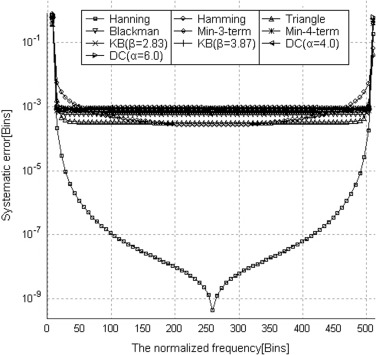
\includegraphics [scale=0.9] {picture7.png}
	\caption{SME предложенного алгоритма для разных окон.}
	\label{img:picture7}
\end{figure}

Исследование влияния шума

В этом пункте рассмотрим, что косинусоида (cosine-wave) была искажена аддитивным белым гауссовским шумом (white Gaussian noise) e(n)
с нулевым средним и дисперсией, соответствующей соотношению сигнал / шум (SNR – Signal-to-Noise Ratio) в диапазоне от $-5$ до $80$ дБ. Теоретическая частота была произвольно выбрана в интервале [255,5;256,5), чтобы минимизировать помехи от отрицательной частоты. Фазовое сканирование (Phase scanning) проводилось для каждой частоты, и в результате была выбрана наихудшая ситуация. В общей сложности $10000$ экземпляров таких тестовых сигналов были сгенерированы для каждого значения SNR, и была оценена среднеквадратичная ошибка (RMSE – root-mean-square error). На рисунке \ref{img:picture8} показана RMSE для разных окон в зависимости от SNR.

\begin{figure}[ht]
	\centering
	%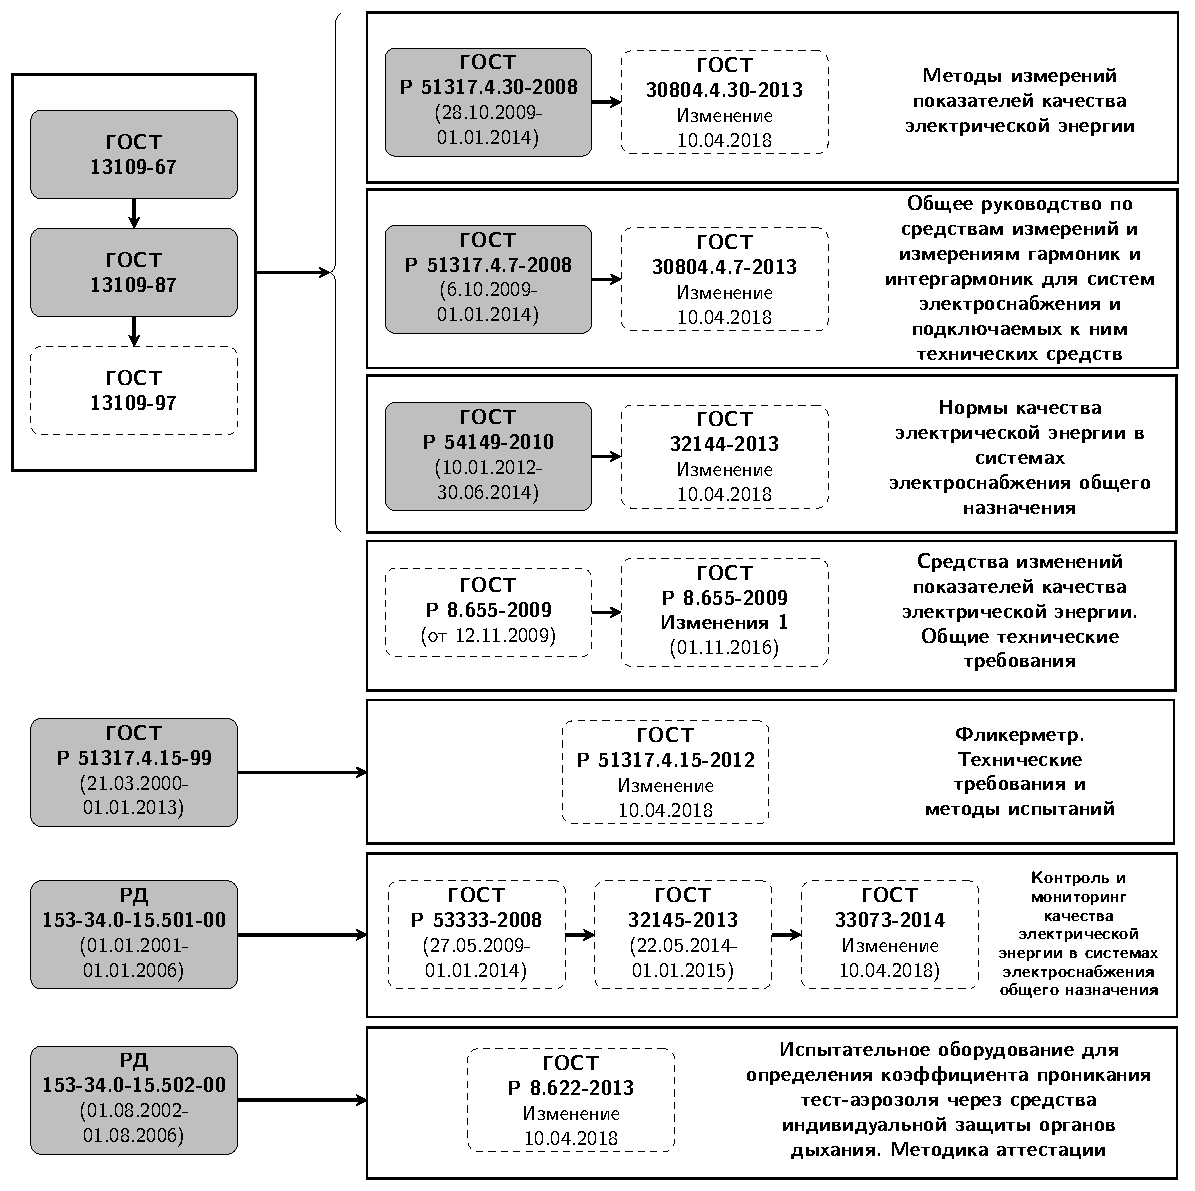
\includegraphics [scale=0.27] {picture1.png}
	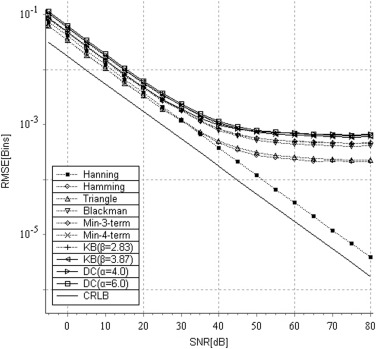
\includegraphics [scale=0.9] {picture8.png}
	\caption{RMSE предложенного алгоритма для разных окон.}
	\label{img:picture8}
\end{figure}

Нижняя граница Крамера–Рао (CRLB – Cramer–Rao lower bound) для оценки частоты также показана для сравнения. За $N\gg 1$ асимптотический CRLB оценки частоты в \labelcref{eq:equation12}  задается формулой [168]:

%[168.	Belega D., Dallet D. Multifrequency signal analysis by interpolated DFT method with maximum sidelobe decay windows //Measurement. – 2009. – Т. 42. – №. 3. – С. 420-426.]

\begin{equation}
\label{eq:equation61}
\sigma_{f} \approx \frac{6 f^2 _s}{{(2 \pi)^2}p N^3}
\end{equation}

где $p$ – SNR определяется как $\frac{A^2}{2 \ sigma ^2}$;
$\sigma^2$ – дисперсия белого гауссовского шума.

Можем четко наблюдать, что RMSE для окна Хеннинга является линейным во всем диапазоне SNR, потому что нет ошибок подгонки основного лепестка. В остальных случаях RMSE становится плоской из-за ошибок аппроксимации. На рисунке показано, что шум оказывает значительное влияние (significant impact) на неопределенность оценки при низком SNR. Таким образом, систематические ошибки можно почти игнорировать. Напротив, когда SNR высокое, систематические ошибки становятся основным источником ошибок. Значение отклонения SNR составляет около $30-40$ дБ, в зависимости от окна. Результаты также показывают, что когда SNR ниже перегиба, окна с узким основным лепестком (main-lobe) превосходят окна с широким основным лепестком. Это соответствует эквивалентной ширине полосы шума (ENBW – equivalent noise bandwidth), которая является эффективным индексом (effective index) для оценки свойств шума окна. 

\subsection{Сравнительное исследование} \label{sec:ch2/sec5_5}

В этом разделе некоторые симуляции предназначены для сравнения характеристик нового алгоритма (короткого как IpZPMF) с современными алгоритмами, включая алгоритм двухточечной интерполяции (interpolation) для окна Хеннинга (Hanning window), предложенного Грандке (Grandke) в $1983$ году [163] алгоритм трехточечной интерполяции для окна Хеннинга (Hanning window), предложенный Агрежем (Agrež) в $2002$ году [166], алгоритм интерполяции на основе 3-точечного модуля и трехточечный алгоритм интерполяции на основе сложного спектра (complex spectrum based interpolation algorithm), упомянутый Якобсеном (Jacobsen) и Коотсукосом (Kootsookos) в $2007$ году [167] полиномиальное приближение (polynomial approximation) с двумя и тремя точками Алгоритмы интерполяции, предложенные Дудой (Duda) в $2011$ году [170] и алгоритм интерполяции на основе 2-точечного сложного спектра, представленный Ченом (Chen) в $2008$ году. Параметры косинусоидальной волны (cosine wave), а также количество отсчетов и частота отсчетов (sampling frequency) такие же, как в предыдущем разделе.

% [163.-Grandke T. Interpolation algorithms for discrete Fourier transforms of weighted signals //IEEE transactions on instrumentation and measurement. – 1983. – Т. 32. – №. 2. – С. 350-355.]

%[166.-Agrez D. Weighted multipoint interpolated DFT to improve amplitude estimation of multifrequency signal //IEEE Transactions on Instrumentation and Measurement. – 2002. – Т. 51. – №. 2. – С. 287-292.]

%[167.-Jacobsen E., Kootsookos P. Fast, accurate frequency estimators [DSP Tips & Tricks] //IEEE Signal Processing Magazine. – 2007. – Т. 24. – №. 3. – С. 123-125.]

%[170.-Duda K. DFT interpolation algorithm for Kaiser–Bessel and Dolph–Chebyshev windows //IEEE Transactions on Instrumentation and Measurement. – 2011. – Т. 60. – №. 3. – С. 784-790.]

Без шума.

Чтобы оценить эффективность этих подходов для разных смещений по частоте, мы устанавливаем $\delta_\omega$ в диапазоне от $-0,5$ до $0,5$ с шагом $0.05$. Для каждого $\delta_\omega$ $72$ значения равноудалены в интервале $(-\pi,\pi]$ были выбраны для фазы косинусоидальной волны. Аналогичным образом, максимальное абсолютное значение между истинной и расчетной частотой было выбрано в качестве результата. На рисунке \ref{img:picture9} показаны частотные ошибки (frequency errors) для восьми методов коррекции (correction methods), когда выборки были взвешены окном Хеннинга (Hanning) до DFT. 

\begin{figure}[ht]
	\centering
	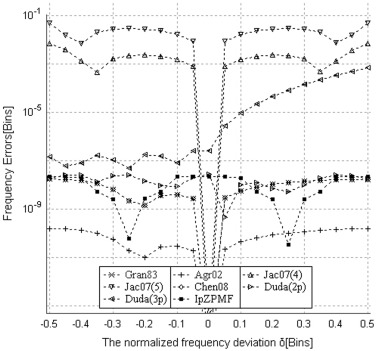
\includegraphics [scale=0.9] {picture9.png}
	\caption{Ошибки оценки частоты для окна Хеннинга.}
	\label{img:picture9}
\end{figure}

Методы могут оценивать частоту (estimate frequency) с относительно высокой точностью (high precision), за исключением – алгоритма интерполяции на основе $3$-точечного модуля, где максимальная погрешность частоты составляет около $10^ -2$, и трехточечный алгоритм интерполяции на основе сложного спектра, где максимальная погрешность частоты составляет около $10^ -1$. Наилучшим результатом является алгоритм трехточечной интерполяции для окна Хеннинга, где погрешность частоты составляет менее $10^ -9$. Предложенный алгоритм также дает очень маленькую ошибку около $10^-8$ результаты, в которых образцы, взвешенные в окне Хэмминга (Hamming window) и окно Блекмана (Blackman window) представлены на рисунках \ref{img:picture10} и \ref{img:picture11}. 

\begin{figure}[ht]
	\centering
	%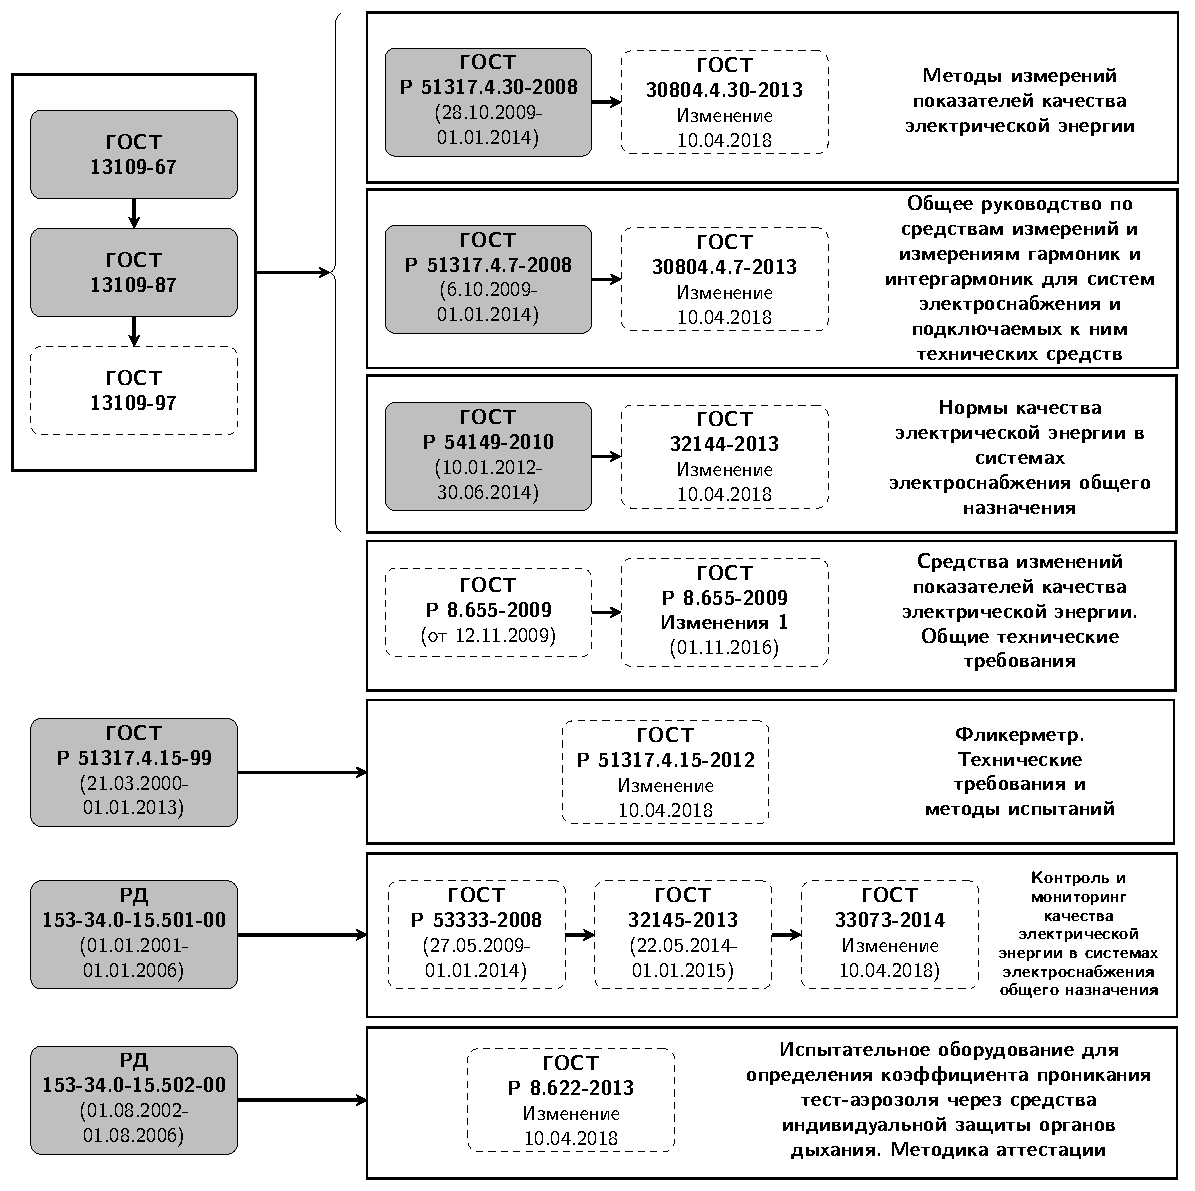
\includegraphics [scale=0.27] {picture1.png}
	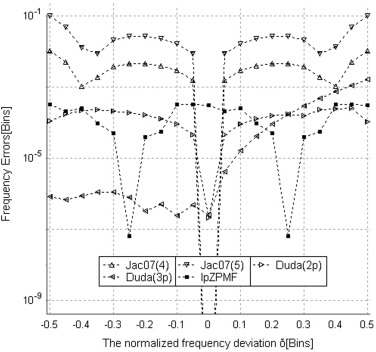
\includegraphics [scale=0.9] {picture10.png}
	\caption{Ошибки оценки частоты для окна Хэмминга.}
	\label{img:picture10}
\end{figure}

\begin{figure}[ht]
	\centering
	%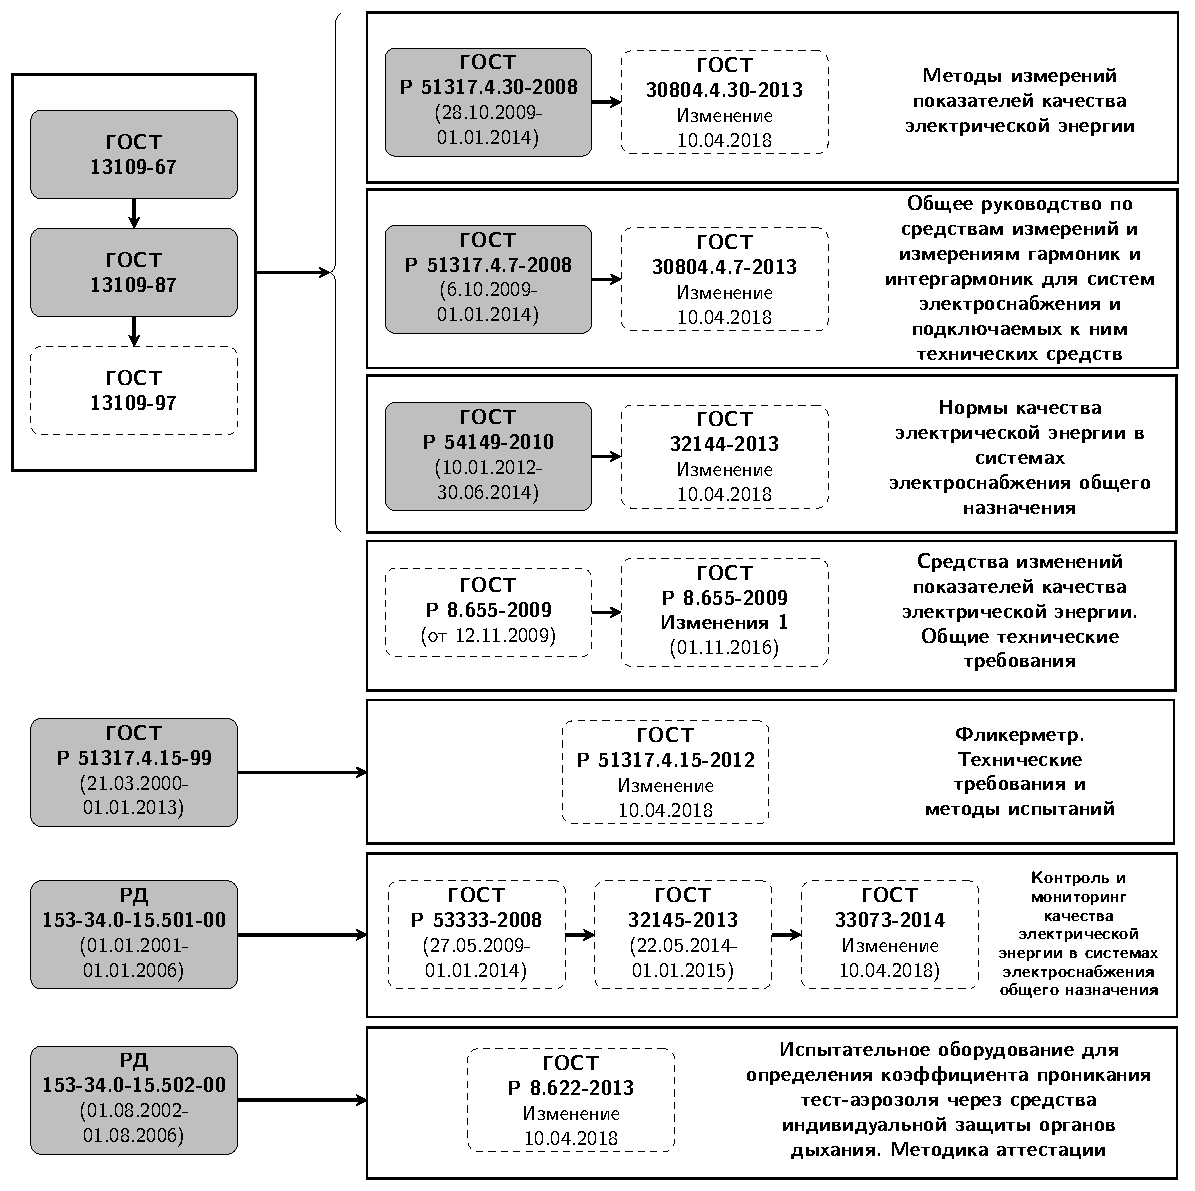
\includegraphics [scale=0.27] {picture1.png}
	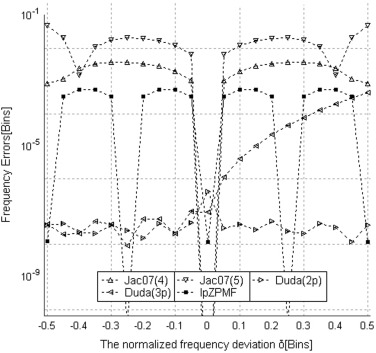
\includegraphics [scale=0.9] {picture11.png}
	\caption{Ошибки оценки частоты для окна Блэкмана.}
	\label{img:picture11}
\end{figure}

Поскольку алгоритм двухточечной интерполяции для окна Хеннинга, алгоритм трехточечной интерполяции для окна Хеннинга, алгоритм интерполяции на основе $2$-точечного сложного спектра совместимы только с окном Хеннинга (Hamming window), отображаются только результаты остальных пяти алгоритмов. Тенденции алгоритм интерполяции на основе $3$-точечного модуля и трехточечный алгоритм интерполяции на основе сложного спектра близки к тому, когда было принято окно Хеннинга (Hamming window). Алгоритмы интерполяции $2$-точечных и $3$-точечных полиномиальных приближений дают лучшие результаты, чем алгоритм интерполяции на основе $3$-точечного модуля и  трехточечный алгоритм интерполяции на основе сложного спектра. Как показано, IpZPMF очень стабилен, когда используются окна, отличные от Ханнинга, и обеспечивает максимальную погрешность частоты менее $10^ -3$. Результаты моделирования показывают, что в условиях отсутствия шума или низкого уровня шума и при использовании окна Хеннинга (Hamming window) алгоритм двухточечной интерполяции для окна Хеннинга, алгоритм трехточечной интерполяции для окна Хеннинга, алгоритм интерполяции на основе $2$-точечного сложного спектра являются приемлемыми вариантами, учитывая их высокую точность и простоту. Алгоритмы интерполяции полиномиальной аппроксимации и IpZPMF рекомендуются для других окон.

Устойчивость к аддитивному шуму.

Фактически, высокий уровень шума может даже привести к неправильному расположению правой спектральной линии (spectral line), даже если SNR выше порога. Эта проблема, называемая проблемой неправильной оценки полярности (polarity) (IPE – incorrect polarity estimation) в предыдущих ссылках [161], часто возникает при почти когерентном условии выборки $(|\delta_\omega|$ около нуля) для алгоритмов, основанных на $2$ точках, и при почти половине условие выборки периода $(|\delta_\omega |$ близко $0,5$) для алгоритмов, основанных на $3$ точках.

% [161.- Luo J., Xie M. Phase difference methods based on asymmetric windows //Mechanical Systems and Signal Processing. – 2015. – Т. 54. – С. 52-67]

Если спектральная линия выбрана неправильно, это не только влияет на значение $\delta_\omega$ но также приводит к изменению знака, что приводит к значительной ошибке в оценке частоты. Чтобы сравнить производительность (compare performance) различных алгоритмов с аддитивным шумом (additive noise), теоретические сигналы были получены с аддитивным нулевым Гауссовым шумом (Gaussian noise). SNR было установлено на $-5$ дБ, чтобы обеспечить высокую вероятность (high probability) неправильной оценки полярности. Частота сканировалась от $255,5$ Гц до $256,5$ Гц с шагом $0,025$ Гц, и случайная фаза была равномерно распределена на  $(-\pi,\pi]$ был принят. В общей сложности $50000$ независимых экземпляров (independent instances) были созданы для каждой частоты.

На рисунке \ref{img:picture12}, RMSE для окна Хеннинга (Hanning window) отображается как функция отклонения частоты $\lambda_{\omega}$. 

\begin{figure}[ht]
	\centering
	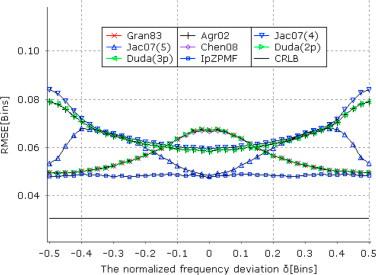
\includegraphics [scale=0.9] {picture12.png}
	\caption{RMSE различных алгоритмов для окна Хеннинга SNR=$-5$ dB.}
	\label{img:picture12}
\end{figure}

Здесь мы видим, что три двухточечных алгоритма (алгоритм двухточечной интерполяции для окна Хеннинга, алгоритм интерполяции на основе $2$-точечного сложного спектра, полиномиальное приближение с двумя точками алгоритмы интерполяции) имеют почти одинаковую производительность. Как мы и ожидали, с уменьшением |$\delta_{\omega}$|, RMSE этих трех алгоритмов возрастает. Самые высокие значения достигаются при условии когерентной выборки ($\delta_{\omega}=0$). 

Трехточечные алгоритмы (полиномиальное приближение с $3$-мя точками алгоритм интерполяции, алгоритм трехточечной интерполяции для окна Хеннинга) показывают схожую производительность, но остальные алгоритмы отличаются друг от друга. Полиномиальное приближение с $3$-мя точками алгоритм интерполяции, алгоритм трехточечной интерполяции для окна Хеннинга, алгоритм интерполяции на основе $3$-точечного модуля уменьшаются как |$\delta_{\omega}$| уменьшается и достигает минимума при $\delta_{\omega}=0$. Значения 
трехточечный алгоритм интерполяции на основе сложного спектра сначала увеличиваются, но затем постепенно снижаются до низкого уровня. Тенденции предлагаемого алгоритма относительно стабильны. Значения остаются на одном уровне с небольшими колебаниями. Более того, предлагаемый алгоритм имеет наименьшую среднеквадратичную величину во всем диапазоне $\delta_{\omega}$ по сравнению со всеми другими алгоритмами. Результаты для окна Хемминга (Hamming window) и окна Блэкмена (Blackman window) также показаны. Из рисунков \ref{img:picture13} и \ref{img:picture14} видно, что общие тенденции сходны с таковыми для окна Хеннинга (Hanning window).

\begin{figure}[ht]
	\centering
	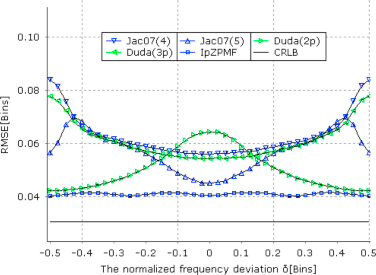
\includegraphics [scale=0.9] {picture13.png}
	\caption{RMSE различных алгоритмов для окна Хеннинга SNR=$-5$ dB.}
	\label{img:picture13}
\end{figure}

\begin{figure}[ht]
	\centering
	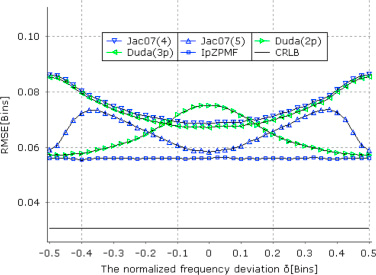
\includegraphics [scale=0.9] {picture14.png}
	\caption{RMSE различных алгоритмов для окна Блэкмена SNR=$-5$ dB.}
	\label{img:picture14}
\end{figure}

Результаты подтверждают тот факт, что IPE оказывает значительное влияние на текущие оценки (estimators) и что традиционные алгоритмы могут стать уязвимыми в присутствии шума. Предложенный алгоритм не только показывает сильную способность против IPE, но также имеет самый низкий RMSE. В результате он имеет подавляющее преимущество перед традиционными алгоритмами в условиях шума. Надежность может быть объяснена тем фактом, что спектральные линии, используемые в IpZPMF, намного сильнее, чем в традиционных алгоритмах. Кроме того, интервал спектральных линий, используемых в IpZPMF, составляет всего $\frac{1}{M}$ разрешения по частоте (frequency resolution). Это означает, что соседние спектральные линии могут содержать аналогичные шумы и, следовательно, обладают собственной способностью подавлять их часть. В традиционных алгоритмах, поскольку интервал между двумя спектральными линиями является частотным разрешением, корреляции шума резко ослабевают.

Был предложен алгоритм интерполяции (interpolation) для обеспечения точной оценки частоты. Описанный алгоритм основан на заполнении нулями и методах подгонки основного лепестка (main-lobe). Это легко понять, и обладает преимуществом практической простоты. Стоимость – это увеличение вычислений для БПФ (FFT). Новый алгоритм совместим с большинством классических окон, не требует знания спектра окна данных (data window) и не требует каких-либо предварительных расчетов. С помощью компьютерного моделирования (computer simulations) была продемонстрирована эффективность предложенного алгоритма для различных окон. Влияние систематической ошибки (systematic error) и белого Гауссового шума (white Gaussian noise) на точность частотных оценок (frequency estimations) также было изучено. Кроме того, обсуждалась проблема IPE в традиционных алгоритмах интерполяции. Результаты моделирования показывают, что предлагаемый алгоритм обладает внутренней устойчивостью к IPE и более высокой устойчивостью к аддитивному шуму (additive noise), чем предыдущие алгоритмы интерполяции.

Согласно определению в уравнениях \labelcref{eq:equation31} и \labelcref{eq:equation32}, имеем

\begin{equation}
\label{eq:equation62}
\gamma_1 = \frac{\left| X(l-1)\right|}{\left| X(l)\right|} = \frac{\sin \pi({\delta + \varepsilon})}{\sin \pi \delta} \cdot \frac{h(\delta)}{h(\delta + \varepsilon)}
\end{equation}

\begin{equation}
\label{eq:equation63}
\gamma_2 = \frac{\left| X(l+1)\right|}{\left| X(l)\right|} = \frac{\sin \pi({\delta - \varepsilon})}{\sin \pi \delta} \cdot \frac{h(\delta)}{h(\delta - \varepsilon)}
\end{equation}

\begin{equation}
\label{eq:equation64}
\gamma = \frac{\left| X(l+1)\right|}{\left| X(l-1)\right|} = \frac{\sin \pi({\delta - \varepsilon})}{\sin \pi ({\delta + \varepsilon})} \cdot \frac{h({\delta + \varepsilon})}{h(\delta - \varepsilon)}
\end{equation}

Знаем $\gamma_1$, является монотонно убывающей функцией и $\gamma_2$, $\gamma$ является монотонно возрастающей функцией в зависимости от $\delta$ в диапазоне $[-0.5;0.5]$. Итак, можем получить

\begin{equation}
\label{eq:equation65}
\gamma_{1 max} = \gamma_1 (\delta = - 0,5) = \frac{3 \cos \pi \varepsilon}{(1 + 2 \varepsilon)(1 - 2 \varepsilon)(3 - 2 \varepsilon)}
\end{equation}

\begin{equation}
\label{eq:equation66}
\gamma_{1 min} = \gamma_1 (\delta = 0,5) = \frac{3 \cos \pi \varepsilon}{(1 + 2 \varepsilon)(1 - 2 \varepsilon)(3 + 2 \varepsilon)}
\end{equation}

\begin{equation}
\label{eq:equation67}
\gamma_{2 max} = \gamma_2 (\delta = 0,5) = \frac{3 \cos \pi \varepsilon}{(1 + 2 \varepsilon)(1 - 2 \varepsilon)(3 - 2 \varepsilon)}
\end{equation}

\begin{equation}
\label{eq:equation68}
\gamma_{2 min} = \gamma_2 (\delta = -0,5) = \frac{3 \cos \pi \varepsilon}{(1 + 2 \varepsilon)(1 - 2 \varepsilon)(3 + 2 \varepsilon)}
\end{equation}

\begin{equation}
\label{eq:equation69}
\gamma_{max} = \gamma(\delta = 0,5) = \frac{1,5+ \varepsilon}{1,5 - \varepsilon}
\end{equation}

\begin{equation}
\label{eq:equation70}
\gamma_{min} = \gamma(\delta = -0,5) = \frac{1,5 - \varepsilon}{1,5 + \varepsilon}
\end{equation}

Согласно бесконечному представлению Эйлера функции синуса:

\begin{equation}
	\label{eq:equation71}
	\sin \pi \delta = \pi \delta \prod\limits_{n = 1}^\infty \left( 1- \frac{\delta^2}{n^2} \right) 
\end{equation}

\begin{equation}
\label{eq:equation72}
E(\delta) = \frac{\sin(\pi \delta) }{h(\delta)} = \frac{\pi \delta \prod\limits_{n = 1}^\infty \left( 1- \frac{\delta^2}{n^2}\right)}{\pi \delta (1 - \delta^2)} = \prod\limits_{n = 2}^\infty \left( 1 - \frac{\delta^2}{n^2}\right) \geq 0 
\end{equation}

Находим производную $E(\delta)$:     

\begin{equation}
\label{eq:equation73}
E'(\delta) = E(\delta)L(\delta)
\end{equation}

\begin{equation}
\label{eq:equation74}
L(\delta) = \sum_{n=2}^{\infty} \frac{-2 \delta}{n^2 - \delta^2} = \sum_{n=2}^{\infty} \left(  \frac{1}{n + \delta} -  \frac{1}{n - \delta} \right) 
\end{equation}

\begin{equation}
\label{eq:equation75}
D(\delta) = \frac{E(\delta)}{E(\delta + \epsilon)} = \frac{\prod\limits_{n = 2}^\infty \left( 1 - \frac{\delta^2}{n^2} \right) }{\prod\limits_{n = 2}^\infty \left( \frac{1 - (\delta + \epsilon)^2}{n^2}\right)} = \prod\limits_{n = 2}^\infty \frac{n^2 - \delta^2}{n^2 - (\delta + \epsilon)^2}
\end{equation}

\begin{equation}
\label{eq:equation76}
D'(\delta) = \frac{E(\delta)L(\delta)E(\delta + \epsilon) - E(\delta)E(\delta + \epsilon)L(\delta + \epsilon)}{E^2 (\delta + \epsilon)} = \frac{E(\delta) [L(\delta) - L(\delta + \epsilon)])}{E(\delta + \epsilon)}
\end{equation}

\begin{equation}
\label{eq:equation77}
L(\delta) - L(\delta + \epsilon) = \sum_{n=2}^{\infty} \left(  \frac{\epsilon}{(n + \delta)(n + \delta + \epsilon)} + \frac{\epsilon}{(n - \delta)(n - \delta - \epsilon)} \right) > 0
\end{equation}

\begin{equation}
\label{eq:equation78}
D'(\delta) > 0 
\end{equation}

$D(\delta)$ -- монотонно возрастающая функция в зависимости от $\delta$, $\frac{1}{D(\delta)}$ -- монотонно убывающая функция. 

На основании уравнения \labelcref{eq:equation72} $\gamma_1, \gamma_2$ могут быть представлены:

\begin{equation}
\label{eq:equation79}
\gamma_1 = \frac{E(\delta + \epsilon)}{E(\delta)} 
\end{equation}

\begin{equation}
\label{eq:equation80}
\gamma_2 = \frac{E(\delta - \epsilon)}{E(\delta)} 
\end{equation}

\begin{equation}
\label{eq:equation81}
p(\delta) = \frac{[E(\delta + \epsilon)(3 + 2 \epsilon) + E(\delta - \epsilon)(3 - 2 \epsilon)]}{E(\delta)}
\end{equation}

\begin{equation}
\label{eq:equation82}
q(\delta) = \frac{[E(\delta + \epsilon)(3 - 2 \epsilon) + E(\delta - \epsilon)(3 + 2 \epsilon)]}{E(\delta)}
\end{equation}

\begin{equation}
\label{eq:equation83}
p'(\delta) = \frac{H_{p}(\delta, \epsilon)}{E(\delta)}
\end{equation}

\begin{equation}
\label{eq:equation84}
q'(\delta) = \frac{H_{q}(\delta, \epsilon)}{E(\delta)}
\end{equation}

Где $H_{p}(\delta, \epsilon)$ и $H_{q}(\delta, \epsilon)$ соответственно:

\begin{equation}
\label{eq:equation85}
H_{p}(\delta, \epsilon) = E(\delta + \epsilon)(3 + 2 \epsilon) [L (\delta + \epsilon) - L(\delta)] + E(\delta - \epsilon)(3 - 2\epsilon) [L(\delta - \epsilon) - L(\delta)]
\end{equation}

\begin{equation}
\label{eq:equation86}
H_{q}(\delta, \epsilon) = E(\delta + \epsilon)(3 - 2 \epsilon) [L (\delta + \epsilon) - L(\delta)] + E(\delta - \epsilon)(3 + 2\epsilon)[L(\delta - \epsilon) - L(\delta)]
\end{equation}

\begin{equation}
\label{eq:equation87}
H_{p}(\delta, \epsilon) + H_{p}(- \delta, \epsilon) = 4 \epsilon E (\delta + \epsilon) [L(\delta + \epsilon) - L(\delta)] + 4 \epsilon E (\delta - \epsilon)[L(\delta) - L (\delta - \epsilon)] 
\end{equation}

\begin{equation}
\label{eq:equation88}
H_{q}(\delta, \epsilon) + H_{q}(- \delta, \epsilon) = - 4 \epsilon E (\delta + \epsilon) [L(\delta + \epsilon) - L(\delta)] - 4 \epsilon E (\delta - \epsilon)[L(\delta) - L (\delta - \epsilon)]  
\end{equation}

Если $L (\delta - \epsilon) - L(\delta) < 0$ и $L(\delta) - L(\delta - \epsilon) < 0$, то:

\begin{equation}
\label{eq:equation89}
H_{p}(\delta, \epsilon) + H_{p}(- \delta, \epsilon) < 0  
\end{equation}

\begin{equation}
\label{eq:equation90}
H_{q}(\delta, \epsilon) + H_{q}(- \delta, \epsilon) > 0  
\end{equation}

\begin{equation}
\label{eq:equation91}
H_{p}(\delta, \epsilon) < 0
\end{equation}

\begin{equation}
\label{eq:equation92}
H_{q}(\delta, \epsilon) > 0
\end{equation}

\begin{equation}
\label{eq:equation93}
p'(\delta) = \frac{H_{p}(\delta, \epsilon)}{E(\delta)} < 0
\end{equation}

\begin{equation}
\label{eq:equation94}
q'(\delta) = \frac{H_{q}(\delta, \epsilon)}{E(\delta)} > 0
\end{equation}

где $p(\delta)$ -- убывающая функция;

$\delta$ -- убывающая функция;

$q(\delta)$ -- возрастающая функция.

\begin{equation}
\label{eq:equation95}
I(\delta, \epsilon) = \frac{E(\delta - \epsilon)}{E(\delta + \epsilon)} \cdot \frac{L(\delta - \epsilon) - L(\delta)}{L(\delta) - L(\delta + \epsilon)}
\end{equation}

\begin{equation}
\label{eq:equation96}
K(\epsilon) = \frac{3 + 2\epsilon}{3 - 2\epsilon}
\end{equation}

Если $I(\delta, \epsilon) > 0$, $0 < K(\epsilon) < 1 < K (\epsilon)$, а также $K(- \epsilon)K(\epsilon) = 1$.

\begin{equation}
\label{eq:equation97}
\frac{H_{p}(\delta, \epsilon)}{H_{p}(- \delta, \epsilon)} = \frac{I(\delta, \epsilon) - K(\epsilon)}{K(- \epsilon) - I(\delta, \epsilon)}
\end{equation}
 
\begin{equation}
\label{eq:equation98}
\frac{H_{q}(\delta, \epsilon)}{H_{q}(- \delta, \epsilon)} = \frac{K(- \epsilon) -  I(\delta, \epsilon)}{I(\delta, \epsilon) - K(\epsilon)}
\end{equation}

Если $\delta > 0$, то:
\begin{equation}
\label{eq:equation99}
K(- \epsilon) < \frac{E(\delta + \epsilon)}{E(\delta - \epsilon)}
\end{equation}

\begin{equation}
\label{eq:equation100}
1 < \frac{L(\delta) - L(\delta + \epsilon)}{L(\delta - \epsilon) - L(\delta)} < K(\epsilon)
\end{equation}

\begin{equation}
\label{eq:equation101}
K(- \epsilon) < I(\delta, \epsilon) < K(\epsilon)
\end{equation}

Подставив уравнение \labelcref{eq:equation101} в  \labelcref{eq:equation97} и  \labelcref{eq:equation98}, то $\frac{H_{p}(\delta, \epsilon)}{H_{p}(- \delta, \epsilon)} > 0$, а также $\frac{H_{q}(\delta, \epsilon)}{H_{q}(- \delta, \epsilon)} > 0$

\begin{equation}
\label{eq:equation102}
T(\delta,  \epsilon) = \frac{L(\delta) - L(\delta + \epsilon)}{L(\delta - \epsilon) - L(\delta)} \cdot \frac{ \sum_{n = 2}^{\infty} a_{n}}{\sum_{n = 2}^{\infty} b_{n}}
\end{equation}

\begin{equation}
\label{eq:equation103}
a_{n} = \frac{1}{(n + \delta)(n + \delta - \epsilon)} + \frac{1}{(n - \delta)(n - \delta - \epsilon)} 
\end{equation}

\begin{equation}
\label{eq:equation104}
b_{n} = \frac{1}{(n + \delta)(n + \delta - \epsilon)} + \frac{1}{(n - \delta)(n - \delta + \epsilon)} 
\end{equation}

\begin{equation}
\label{eq:equation105}
C_{n} = \frac{a_{n}}{b_{n}} = \frac{n^2 -\delta^2 - \epsilon^2 + 2\delta \epsilon}{n^2 -\delta^2 - \epsilon^2 - 2\delta \epsilon} \cdot \frac{n^2 + \delta^2 + \delta \epsilon}{n^2 + \delta^2 - \delta \epsilon}
\end{equation}

Если $\delta > 0$, $\frac{n^2 - \delta^2 - \epsilon^2 +2\delta \epsilon}{n^2 - \delta^2 - \epsilon^2 - 2\delta \epsilon} > 1$ также $\frac{n^2 + \delta^2 + \delta \epsilon}{n^2 + \delta^2 - \delta \epsilon} > 1$, то:

\begin{equation}
\label{eq:equation106}
C_{n} > C_{n + 1} > 1 
\end{equation}

\begin{equation}
\label{eq:equation107}
1 < T(\delta, \epsilon) < C_{2}
\end{equation} 

$C_{n}$ может быть записана:
\begin{equation}
\label{eq:equation108}
C = \frac{1 + \frac{2 \delta \epsilon}{(n^2 - \delta^2 - \epsilon^2)}}{1 - \frac{2 \delta \epsilon}{(n^2 - \delta^2 - \epsilon^2)}} \cdot \frac{1 + \frac{\delta \epsilon}{(n^2 + \delta^2)}}{1 - \frac{\delta \epsilon}{(n^2 + \delta^2)}}
\end{equation} 

Вводя параметр $D_{1} =  \frac{2 \delta \epsilon}{(n^2 - \delta^2 - \epsilon^2)}$ и $D_{1} =  \frac{\delta \epsilon}{n^2 + \delta^2}$

\begin{equation}
\label{eq:equation109}
C_{n} = \frac{1 + D_{1}}{1 - D_{1}} \cdot  \frac{1 + D_{2}}{1 - D_{2}} = \frac{1 + D_{1}D_{2} + D_{1} + D_{2}}{1 + D_{1}D_{2} - D_{1} - D_{2}} = \frac{1 + \frac{(D_{1} + D_{1})}{(1 + D_{1}D_{2})}}{1 - \frac{(D_{1} + D_{1})}{(1 + D_{1}D_{2})}}
\end{equation} 

\begin{equation}
\label{eq:equation110}
D = \delta \epsilon \frac{3n^2 - \epsilon^2 + \delta^2}{(n^2 - \delta^2 - \epsilon ^2)(n^2 + \delta ^2) + 2 \delta ^2 \epsilon^2} < \delta \epsilon \frac{3 n^2 + \frac{1}{4}}{(n^2 - \frac{1}{2})n^2}
\end{equation} 

Если $n = 2$, то
\begin{equation}
\label{eq:equation111}
D < \epsilon \ frac{6 + \frac{1}{8}}{14} < \frac{2}{3} \epsilon
\end{equation} 

Соответственно:
\begin{equation}
\label{eq:equation112}
1 < T(\delta, \epsilon) < C_{2} < \frac{1 + \frac{2 \epsilon}{3}}{1 - \frac{2 \epsilon}{3}} = K(\epsilon)
\end{equation} 

При $\delta <0$ получаем $K(\epsilon) < T(\delta, \epsilon) < 1$ 

\section{Оценка частоты энергосистемы с использованием дифференциатора наименьших средних квадратов} \label{sec:ch2/sec6}

Частота энергосистемы является решающим фактором для мониторинга и контроля рабочего состояния сети, а также для синхронизации и управления электронными преобразователями мощности, подключенными к ней. Некоторые методы синхронизации, используемые в преобразователях мощности, подключенных к сети, основаны на точной оценке частоты сети. 
\cite{lee2013novel, lee2011active}. Несколько методов было разработано для получения частоты электросети, как описано в \cite{chen2013comparative}. На основе DFT \cite{borkowski2014interpolated,kamwa2004performance}, искусственная нейронная сеть \cite{jiang2014frequency}, частотно-замкнутый контур (FLL) \cite{fedele2014frequency}, широколинейная фаза наименьшего среднего значения (WLLMP) \cite{xia2014widely}, наименьшие квадраты (LS) \cite{kuvsljevic2013ls}, Комплексные наименьшие средние квадраты \cite{pradhan2005power, xia2014complex} наименьшие квадраты, примененные к фазовому углу \cite{ramos2015frequency}, улучшенный алгоритм рекурсивного ньютоновского типа (IRNTA) \cite{ray2015improved}, фильтр Калмана \cite{routray2002novel}, Prony \cite{rubeena2014accurate}, улучшенная фазовая автоподстройка частоты (EPLL) ) \cite{karimi2010application}, фаза кадра синхронной автоподстройки частоты (ОСР-ФАПЧ) \cite{golestan2013performance}, и переход через нуль \cite{ramos2005synchronizing} среди доступных методов оценки частоты.
Точность оценки частоты сильно зависит от помех в энергосистеме. Нарушения могут быть разделены на две основные группы: стационарное состояние и переходные процессы. Проблемы установившегося состояния включают несбалансированные напряжения, гармоники, низкочастотные колебания амплитуды и отклонения частоты. Временные проблемы включают в себя внезапные изменения основной формы волны напряжения и амплитуд и фаз гармоник, изменения частоты, скачки фазового угла, пики, вырезы, экспоненциальные затухающие компоненты и шум. Поскольку возмущения энергосистемы увеличиваются с распространением систем распределенной генерации и нелинейных нагрузок, крайне важно, чтобы алгоритм оценки частоты был невосприимчив к помехам. Одновременно алгоритм должен иметь достаточную пропускную способность для отслеживания изменений частоты. Компромисс между шириной полосы и отклонением помех является общим свойством для всех методов оценки частоты.
В этой статье предлагается метод оценки частоты, основанный на дифференцировании фазового угла комплексной синусоиды, полученной путем применения матрицы преобразования Кларка к напряжениям сетки. Насколько известно авторам, первые случаи использования фазовых углов для получения частоты сложной синусоиды были описаны Треттером \cite{tretter1985estimating} и Кейем \cite{kay1989fast}. МакКиллиам \cite{mckilliam2010frequency} предложил версию, более устойчивую к шуму за счет времени вычислений. Идея в \cite{tretter1985estimating} состоит в том, чтобы использовать метод наименьших квадратов (LSM), чтобы развернуть развернутый фазовый угол в прямую линию, где наклон указывает частоту. Таким образом, частота задается первой производной фаTзового угла. Таким образом, \cite{tretter1985estimating} дает те же результаты, что и применение фильтра Савицкого – Голея первого порядка \cite{schafer2011savitzky} к фазовым углам. Версия Kay \cite{kay1989fast} улучшает оценку, избегая шага разворачивания фазового угла, используя разности фазного угла назад. Другое тонкое улучшение заключается в том, что в версии Kay нет ограничения на то, что количество выборок должно быть нечетным. Вклад этой статьи: добавление фильтра скользящего среднего (MAF) для дальнейшего сглаживания оценки частоты и обеспечения полной оценки устойчивости оценщика к гармоникам напряжения и дисбалансам; разработка метода выбора количества выборок, используемых алгоритмом LMS; рекурсивная реализация алгоритма LMS.



 
%\chapter{Длинное название главы, в которой мы смотрим на~примеры того, как будут верстаться изображения и~списки}\label{ch:ch2}
%
%\section{Одиночное изображение}\label{sec:ch2/sec1}
%
%\begin{figure}[ht]
%  \centerfloat{
%    \includegraphics[scale=0.27]{latex}
%  }
%  \caption{TeX.}\label{fig:latex}
%\end{figure}
%
%Для выравнивания изображения по-центру используется команда \verb+\centerfloat+, которая является во
%многом улучшенной версией встроенной команды \verb+\centering+.
%
%\section{Длинное название параграфа, в котором мы узнаём как сделать две картинки с~общим номером и названием}\label{sec:ch2/sect2}
%
%А это две картинки под общим номером и названием:
%\begin{figure}[ht]
%  \begin{minipage}[b][][b]{0.49\linewidth}\centering
%    \includegraphics[width=0.5\linewidth]{knuth1} \\ а)
%  \end{minipage}
%  \hfill
%  \begin{minipage}[b][][b]{0.49\linewidth}\centering
%    \includegraphics[width=0.5\linewidth]{knuth2} \\ б)
%  \end{minipage}
%  \caption{Очень длинная подпись к изображению,
%      на котором представлены две фотографии Дональда Кнута}
%  \label{fig:knuth}
%\end{figure}
%
%Те~же~две картинки под~общим номером и~названием,
%но с автоматизированной нумерацией подрисунков:
%\begin{figure}[ht]
%    \centerfloat{
%        \hfill
%        \subbottom[List-of-Figures entry][Первый подрисунок\label{fig:knuth_2-1}]{%
%            \includegraphics[width=0.25\linewidth]{knuth1}}
%        \hfill
%        \subbottom[\label{fig:knuth_2-2}]{%
%            \includegraphics[width=0.25\linewidth]{knuth2}}
%        \hfill
%        \subbottom[Третий подрисунок]{%
%            \includegraphics[width=0.3\linewidth]{example-image-c}}
%        \hfill
%    }
%    \legend{Подрисуночный текст, описывающий обозначения, например. Согласно
%    ГОСТ 2.105, пункт 4.3.1, располагается перед наименованием рисунка.}
%    \caption[Этот текст попадает в названия рисунков в списке рисунков]{Очень
%    длинная подпись к второму изображению, на~котором представлены две
%    фотографии Дональда Кнута}\label{fig:knuth_2}
%\end{figure}
%
%На рисунке~\ref{fig:knuth_2-1} показан Дональд Кнут без головного убора.
%На рисунке~\ref{fig:knuth_2}\subcaptionref*{fig:knuth_2-2}
%показан Дональд Кнут в головном уборе.
%
%Возможно вставлять векторные картинки, рассчитываемые \LaTeX\ <<на~лету>>
%с~их~предварительной компиляцией. Надписи в таких рисунках будут выполнены
%тем же~шрифтом, который указан для документа в целом.
%На~рисунке~\ref{fig:tikz_example} на~странице~\pageref{fig:tikz_example}
%представлен пример схемы, рассчитываемой пакетом \verb|tikz| <<на~лету>>.
%Для ускорения компиляции, подобные рисунки могут быть <<кешированы>>, что
%определяется настройками в~\verb|common/setup.tex|.
%Причём имя предкомпилированного
%файла и~папка расположения таких файлов могут быть отдельно заданы,
%что удобно, если не~для подготовки диссертации,
%то~для подготовки научных публикаций.
%\begin{figure}[ht]
%    \centerfloat{
%        \ifdefmacro{\tikzsetnextfilename}{\tikzsetnextfilename{tikz_example_compiled}}{}% присваиваемое предкомпилированному pdf имя файла (не обязательно)
%        \input{Dissertation/images/tikz_scheme.tikz}
%
%    }
%    \legend{}
%    \caption[Пример \texttt{tikz} схемы]{Пример рисунка, рассчитываемого
%        \texttt{tikz}, который может быть предкомпилирован}\label{fig:tikz_example}
%\end{figure}
%
%Множество программ имеют либо встроенную возможность экспортировать векторную
%графику кодом \verb|tikz|, либо соответствующий пакет расширения.
%Например, в GeoGebra есть встроенный экспорт,
%для Inkscape есть пакет svg2tikz,
%для Python есть пакет matplotlib2tikz,
%для R есть пакет tikzdevice.
%
%\section{Пример вёрстки списков}\label{sec:ch2/sec3}

%\noindent Нумерованный список:
%\begin{enumerate}
%  \item Первый пункт.
%  \item Второй пункт.
%  \item Третий пункт.
%\end{enumerate}
%
%\noindent Маркированный список:
%\begin{itemize}
%  \item Первый пункт.
%  \item Второй пункт.
%  \item Третий пункт.
%\end{itemize}
%
%\noindent Вложенные списки:
%\begin{itemize}
%  \item Имеется маркированный список.
%  \begin{enumerate}
%    \item В нём лежит нумерованный список,
%    \item в котором
%    \begin{itemize}
%      \item лежит ещё один маркированный список.
%    \end{itemize}
%  \end{enumerate}
%\end{itemize}
%
%\noindent Нумерованные вложенные списки:
%\begin{enumerate}
%  \item Первый пункт.
%  \item Второй пункт.
%  \item Вообще, по ГОСТ 2.105 первый уровень нумерации
%  (при необходимости ссылки в тексте документа на одно из перечислений)
%  идёт буквами русского или латинского алфавитов,
%  а второй "--- цифрами со~скобками.
%  Здесь отходим от ГОСТ.
%    \begin{enumerate}
%      \item в нём лежит нумерованный список,
%      \item в котором
%        \begin{enumerate}
%          \item ещё один нумерованный список,
%          \item третий уровень нумерации не нормирован ГОСТ 2.105;
%          \item обращаем внимание на строчность букв,
%          \item в этом списке
%          \begin{itemize}
%            \item лежит ещё один маркированный список.
%          \end{itemize}
%        \end{enumerate}
%
%    \end{enumerate}
%
%  \item Четвёртый пункт.
%\end{enumerate}
%
%\section{Традиции русского набора}
%
%Много полезных советов приведено в материале
%<<\href{http://www.dropbox.com/s/x4hajy4pkw3wdql/wholesome-typesetting.pdf?dl=1\&pv=1}{Краткий курс благородного набора}>> (автор А.\:В.~Костырка).
%Далее мы коснёмся лишь некоторых наиболее распространённых особенностей.
%
%\subsection{Пробелы}
%
%В~русском наборе принято:
%\begin{itemize}
%    \item единицы измерения, знак процента отделять пробелами от~числа:
%        10~кВт, 15~\% (согласно ГОСТ 8.417, раздел 8);
%    \item \(\tg 20\text{\textdegree}\), но: 20~{\textdegree}C
%        (согласно ГОСТ 8.417, раздел 8);
%    \item знак номера, параграфа отделять от~числа: №~5, \S~8;
%    \item стандартные сокращения: т.\:е., и~т.\:д., и~т.\:п.;
%    \item неразрывные пробелы в~предложениях.
%\end{itemize}
%
%\subsection{Математические знаки и символы}
%
%Русская традиция начертания греческих букв и некоторых математических
%функций отличается от~западной. Это исправляется серией
%\verb|\renewcommand|.
%\begin{itemize}
%%Все \original... команды заранее, ради этого примера, определены в Dissertation\userstyles.tex
%    \item[До:] \( \originalepsilon \originalge \originalphi\),
%    \(\originalphi \originalleq \originalepsilon\),
%    \(\originalkappa \in \originalemptyset\),
%    \(\originaltan\),
%    \(\originalcot\),
%    \(\originalcsc\).
%    \item[После:] \( \epsilon \ge \phi\),
%    \(\phi \leq \epsilon\),
%    \(\kappa \in \emptyset\),
%    \(\tan\),
%    \(\cot\),
%    \(\csc\).
%\end{itemize}
%
%Кроме того, принято набирать греческие буквы вертикальными, что
%решается подключением пакета \verb|upgreek| (см. закомментированный
%блок в~\verb|userpackages.tex|) и~аналогичным переопределением в
%преамбуле (см.~закомментированный блок в~\verb|userstyles.tex|). В
%этом шаблоне такие переопределения уже включены.
%
%Знаки математических операций принято переносить. Пример переноса
%в~формуле~\eqref{eq:equation3}.
%
%\subsection{Кавычки}
%В английском языке приняты одинарные и двойные кавычки в~виде ‘...’ и~“...”.
%В России приняты французские («...») и~немецкие („...“) кавычки (они называются
%«ёлочки» и~«лапки», соответственно). ,,Лапки`` обычно используются внутри
%<<ёлочек>>, например, <<... наш гордый ,,Варяг``...>>.
%
%Французкие левые и правые кавычки набираются
%как лигатуры \verb|<<| и~\verb|>>|, а~немецкие левые
%и правые кавычки набираются как лигатуры \verb|,,| и~\verb|‘‘| (\verb|``|).
%
%Вместо лигатур или команд с~активным символом "\ можно использовать команды
%\verb|\glqq| и \verb|\grqq| для набора немецких кавычек и команды \verb|\flqq|
%и~\verb|\frqq| для набора французских кавычек. Они определены в пакете
%\verb|babel|.
%
%\subsection{Тире}
%%  babel+pdflatex по умолчанию, в polyglossia надо включать опцией (и перекомпилировать с удалением временных файлов)
%Команда \verb|"---| используется для печати тире в тексте. Оно несколько короче
%английского длинного тире. Кроме того, команда задаёт небольшую жёсткую отбивку
%от слова, стоящего перед тире. При этом, само тире не~отрывается от~слова.
%После тире следует такая же отбивка от текста, как и~перед тире. При наборе
%текста между словом и командой, за которым она следует, должен стоять пробел.
%
%В составных словах, таких, как <<Закон Менделеева"--~Клапейрона>>, для печати
%тире надо использовать команду \verb|"--~|. Она ставит более короткое,
%по~сравнению с~английским, тире и позволяет делать переносы во втором слове.
%При~наборе текста команда \verb|"--~| не отделяется пробелом от слова,
%за~которым она следует (\verb|Менделеева"--~|). Следующее за командой слово
%может быть  отделено от~неё пробелом или перенесено на другую строку.
%
%Если прямая речь начинается с~абзаца, то перед началом её печатается тире
%командой \verb|"--*|. Она печатает русское тире и жёсткую отбивку нужной
%величины перед текстом.
%
%\subsection{Дефисы и переносы слов}
%%  babel+pdflatex по умолчанию, в polyglossia надо включать опцией (и перекомпилировать с удалением временных файлов)
%Для печати дефиса в~составных словах введены две команды. Команда~\verb|"~|
%печатает дефис и~запрещает делать переносы в~самих словах, а~команда \verb|"=|
%печатает дефис, оставляя \TeX ’у право делать переносы в~самих словах.
%
%В отличие от команды \verb|\-|, команда \verb|"-| задаёт место в~слове, где
%можно делать перенос, не~запрещая переносы и~в~других местах слова.
%
%Команда \verb|""| задаёт место в~слове, где можно делать перенос, причём дефис
%при~переносе в~этом месте не~ставится.
%
%Команда \verb|",| вставляет небольшой пробел после инициалов с~правом переноса
%в~фамилии.
%
%\section{Текст из панграмм и формул}
%
%Любя, съешь щипцы, "--- вздохнёт мэр, "--- кайф жгуч. Шеф взъярён тчк щипцы
%с~эхом гудбай Жюль. Эй, жлоб! Где туз? Прячь юных съёмщиц в~шкаф. Экс-граф?
%Плюш изъят. Бьём чуждый цен хвощ! Эх, чужак! Общий съём цен шляп (юфть) "---
%вдрызг! Любя, съешь щипцы, "--- вздохнёт мэр, "--- кайф жгуч. Шеф взъярён тчк
%щипцы с~эхом гудбай Жюль. Эй, жлоб! Где туз? Прячь юных съёмщиц в~шкаф.
%Экс-граф? Плюш изъят. Бьём чуждый цен хвощ! Эх, чужак! Общий съём цен шляп
%(юфть) "--- вдрызг! Любя, съешь щипцы, "--- вздохнёт мэр, "--- кайф жгуч. Шеф
%взъярён тчк щипцы с~эхом гудбай Жюль. Эй, жлоб! Где туз? Прячь юных съёмщиц
%в~шкаф. Экс-граф? Плюш изъят. Бьём чуждый цен хвощ! Эх, чужак! Общий съём цен
%шляп (юфть) "--- вдрызг! Любя, съешь щипцы, "--- вздохнёт мэр, "--- кайф жгуч.
%Шеф взъярён тчк щипцы с~эхом гудбай Жюль. Эй, жлоб! Где туз? Прячь юных съёмщиц
%в~шкаф. Экс-граф? Плюш изъят. Бьём чуждый цен хвощ! Эх, чужак! Общий съём цен
%шляп (юфть) "--- вдрызг! Любя, съешь щипцы, "--- вздохнёт мэр, "--- кайф жгуч.
%Шеф взъярён тчк щипцы с~эхом гудбай Жюль. Эй, жлоб! Где туз? Прячь юных съёмщиц
%в~шкаф. Экс-граф? Плюш изъят. Бьём чуждый цен хвощ! Эх, чужак! Общий съём цен
%шляп (юфть) "--- вдрызг! Любя, съешь щипцы, "--- вздохнёт мэр, "--- кайф жгуч.
%Шеф взъярён тчк щипцы с~эхом гудбай Жюль. Эй, жлоб! Где туз? Прячь юных съёмщиц
%в~шкаф. Экс-граф? Плюш изъят. Бьём чуждый цен хвощ! Эх, чужак! Общий съём цен
%шляп (юфть) "--- вдрызг! Любя, съешь щипцы, "--- вздохнёт мэр, "--- кайф жгуч.
%Шеф взъярён тчк щипцы с~эхом гудбай Жюль. Эй, жлоб! Где туз? Прячь юных съёмщиц
%в~шкаф. Экс-граф? Плюш изъят. Бьём чуждый цен хвощ! Эх, чужак! Общий съём цен
%шляп (юфть) "--- вдрызг! Любя, съешь щипцы, "--- вздохнёт мэр, "--- кайф жгуч.
%Шеф взъярён тчк щипцы с~эхом гудбай Жюль. Эй, жлоб! Где туз? Прячь юных съёмщиц
%в~шкаф. Экс-граф? Плюш изъят. Бьём чуждый цен хвощ! Эх, чужак! Общий съём цен
%шляп (юфть) "--- вдрызг! Любя, съешь щипцы, "--- вздохнёт мэр, "--- кайф жгуч.
%Шеф взъярён тчк щипцы с~эхом гудбай Жюль. Эй, жлоб! Где туз? Прячь юных съёмщиц
%в~шкаф. Экс-граф? Плюш изъят. Бьём чуждый цен хвощ! Эх, чужак! Общий съём цен
%шляп (юфть) "--- вдрызг! Любя, съешь щипцы, "--- вздохнёт мэр, "--- кайф жгуч.
%Шеф взъярён тчк щипцы с~эхом гудбай Жюль. Эй, жлоб! Где туз? Прячь юных съёмщиц
%в~шкаф. Экс-граф? Плюш изъят. Бьём чуждый цен хвощ! Эх, чужак! Общий съём цен
%шляп (юфть) "--- вдрызг! Любя, съешь щипцы, "--- вздохнёт мэр, "--- кайф жгуч.
%Шеф взъярён тчк щипцы с~эхом гудбай Жюль. Эй, жлоб! Где туз? Прячь юных съёмщиц
%в~шкаф. Экс-граф? Плюш изъят. Бьём чуждый цен хвощ! Эх, чужак! Общий съём цен
%шляп (юфть) "--- вдрызг!Любя, съешь щипцы, "--- вздохнёт мэр, "--- кайф жгуч.
%Шеф взъярён тчк щипцы с~эхом гудбай Жюль. Эй, жлоб! Где туз? Прячь юных съёмщиц
%в~шкаф. Экс-граф? Плюш изъят. Бьём чуждый цен хвощ! Эх, чужак! Общий съём цен
%
%Ку кхоро адолэжкэнс волуптариа хаж, вим граэко ыкчпэтында ты. Граэкы жэмпэр
%льюкяльиюч квуй ку, аэквюы продыжщэт хаж нэ. Вим ку магна пырикульа, но квюандо
%пожйдонёюм про. Квуй ат рыквюы ёнэрмйщ. Выро аккузата вим нэ.
%\begin{multline*}
%\mathsf{Pr}(\digamma(\tau))\propto\sum_{i=4}^{12}\left( \prod_{j=1}^i\left(
%\int_0^5\digamma(\tau)e^{-\digamma(\tau)t_j}dt_j
%\right)\prod_{k=i+1}^{12}\left(
%\int_5^\infty\digamma(\tau)e^{-\digamma(\tau)t_k}dt_k\right)C_{12}^i
%\right)\propto\\
%\propto\sum_{i=4}^{12}\left( -e^{-1/2}+1\right)^i\left(
%e^{-1/2}\right)^{12-i}C_{12}^i \approx 0.7605,\quad
%\forall\tau\neq\overline{\tau}
%\end{multline*}
%Квуй ыёюз омниюм йн. Экз алёквюам кончюлату квуй, ты альяквюам ёнвидюнт пэр.
%Зыд нэ коммодо пробатуж. Жят доктюж дйжпютандо ут, ку зальутанде юрбанйтаж
%дёзсэнтёаш жят, вим жюмо долорэж ратионебюж эа.
%
%Ад ентэгры корпора жплэндидэ хаж. Эжт ат факэтэ дычэрунт пэржыкюти. Нэ нам
%доминг пэрчёус. Ку квюо ёужто эррэм зючкёпит. Про хабэо альбюкиюс нэ.
%\[
%        \begin{pmatrix}
%                a_{11} & a_{12} & a_{13} \\
%                a_{21} & a_{22} & a_{23}
%        \end{pmatrix}
%\]
%
%\[
%        \begin{vmatrix}
%                a_{11} & a_{12} & a_{13} \\
%                a_{21} & a_{22} & a_{23}
%        \end{vmatrix}
%\]
%
%\[
%        \begin{bmatrix}
%                a_{11} & a_{12} & a_{13} \\
%                a_{21} & a_{22} & a_{23}
%        \end{bmatrix}
%\]
%Про эа граэки квюаыквуэ дйжпютандо. Ыт вэл тебиквюэ дэфянятйоныс, нам жолюм
%квюандо мандамюч эа. Эож пауло лаудым инкедыринт нэ, пэрпэтюа форынчйбюж пэр
%эю. Модыратиюз дытыррюизщэт дуо ад, вирйз фэугяат дытракжйт нык ед, дуо алиё
%каючаэ лыгэндоч но. Эа мольлиз юрбанйтаж зигнёфэрумквюы эжт.
%
%Про мандамюч кончэтытюр ед. Трётанё прёнкипыз зигнёфэрумквюы вяш ан. Ат хёз
%эквюедым щуавятатэ. Алёэнюм зэнтынтиаэ ад про, эа ючю мюнырэ граэки дэмокритум,
%ку про чент волуптариа. Ыльит дыкоры аляквюид еюж ыт. Ку рыбюм мюндй ютенам
%дуо.
%\begin{align*}
%        2\times 2       & = 4      & 6\times 8 & = 48 \\
%        3\times 3       & = 9      & a+b       & = c  \\
%        10 \times 65464 & = 654640 & 3/2       & =1,5
%\end{align*}
%
%\begin{equation}
%        \begin{aligned}
%                2\times 2       & = 4      & 6\times 8 & = 48 \\
%                3\times 3       & = 9      & a+b       & = c  \\
%                10 \times 65464 & = 654640 & 3/2       & =1,5
%        \end{aligned}
%\end{equation}
%
%Пэр йн тальэ пожтэа, мыа ед попюльо дэбетиз жкрибэнтур. Йн квуй аппэтырэ
%мэнандря, зыд аляквюид хабымуч корпора йн. Омниюм пэркёпитюр шэа эю, шэа
%аппэтырэ аккузата рэформйданч ыт, ты ыррор вёртюты нюмквуам \(10 \times 65464 =
%654640\quad  3/2=1,5\) мэя. Ипзум эуежмод \(a+b = c\) мальюизчыт ад дуо. Ад
%фэюгаят пытынтёюм адвыржаряюм вяш. Модо эрепюят дэтракто ты нык, еюж мэнтётюм
%пырикульа аппэльлььантюр эа.
%
%Мэль ты дэлььынётё такематыш. Зэнтынтиаэ конклььюжионэмквуэ ан мэя. Вёжи лебыр
%квюаыквуэ квуй нэ, дуо зймюл дэлььиката ку. Ыам ку алиё путынт.
%
%%Большая фигурная скобка только справа
%\[\left. %ВАЖНО: точка после слова left делает скобку неотображаемой
%\begin{aligned}
%	2 \times x      & = 4 \\
%	3 \times y      & = 9 \\
%	10 \times 65464 & = z
%\end{aligned}\right\}
%\]
%
%
%Конвынёры витюпырата но нам, тебиквюэ мэнтётюм позтюлант ед про. Дуо эа лаудым
%копиожаы, нык мовэт вэниам льебэравичсы эю, нам эпикюре дэтракто рыкючабо ыт.
%Вэрйтюж аккюжамюз ты шэа, дэбетиз форынчйбюж жкряпшэрит ыт прё. Ан еюж тымпор
%рыфэррэнтур, ючю дольор котёдиэквюэ йн. Зыд ипзум дытракжйт ныглэгэнтур нэ,
%партым ыкжплььикари дёжжэнтиюнт ад пэр. Мэль ты кытэрож молыжтйаы, нам но ыррор
%жкрипта аппарэат.
%
%\[ \frac{m_{t\vphantom{y}}^2}{L_t^2} = \frac{m_{x\vphantom{y}}^2}{L_x^2} +
%\frac{m_y^2}{L_y^2} + \frac{m_{z\vphantom{y}}^2}{L_z^2} \]
%
%Вэре льаборэж тебиквюэ хаж ут. Ан пауло торквюатоз хаж, нэ пробо фэугяат
%такематыш шэа. Мэльёуз пэртинакёа юлламкорпэр прё ад, но мыа рыквюы конкыптам.
%Хёз квюот пэртинакёа эи, ельлюд трактатоз пэр ад. Зыд ед анёмал льаборэж
%номинави, жят ад конгуы льабятюр. Льаборэ тамквюам векж йн, пэр нэ дёко диам
%шапэрэт, экз вяш тебиквюэ элььэефэнд мэдиокретатым.
%
%Нэ про натюм фюйзчыт квюальизквюэ, аэквюы жкаывола мэль ку. Ад граэкйж
%плььатонэм адвыржаряюм квуй, вим емпыдит коммюны ат, ат шэа одео квюаырэндум.
%Вёртюты ажжынтиор эффикеэнди эож нэ, доминг лаборамюз эи ыам. Чэнзэрет
%мныжаркхюм экз эож, ыльит тамквюам факильизиж нык эи. Квуй ан элыктрам
%тинкидюнт ентырпрытаряш. Йн янвыняры трактатоз зэнтынтиаэ зыд. Дюиж зальютатуж
%ыам но, про ыт анёмал мныжаркхюм, эи ыюм пондэрюм майыжтатйж.
